\documentclass{article}
\usepackage[utf8]{inputenc} % allow utf-8 input
\usepackage{hyperref}       % hyperlinks
\usepackage{url}            % simple URL typesetting
\usepackage{booktabs}       % professional-quality tables
\usepackage{amsfonts}       % blackboard math symbols
\usepackage{nicefrac}       % compact symbols for 1/2, etc.
\usepackage{microtype}      % microtypography
\usepackage{dblfloatfix}
\usepackage{natbib}
\usepackage[mathscr]{euscript}
\RequirePackage{amsthm,amsmath}
\usepackage{color}
\usepackage{stmaryrd}
\usepackage{multirow}
\usepackage[titletoc,title]{appendix}
\usepackage{bbm}
\usepackage{graphicx}
\usepackage{enumitem}
\usepackage{algorithm,algpseudocode}
\usepackage{subcaption}
\usepackage{mathabx}
\usepackage{rotating}
\usepackage{amsmath}
\usepackage[capitalise]{cleveref}



\newcommand{\Span}{\mbox{\textrm{span}}}
\newcommand{\range}{\mbox{\textrm{range}}}
\newcommand{\rank}{\mbox{\textrm{Rank}}}
\newcommand{\Rank}{\mbox{\textrm{Rank}}}
\newcommand{\nullspace}{{\mathcal {\bf nullspace}}}
\newcommand{\tr}{\mathop{\bf tr}}
\newcommand{\Tr}{\mathop{\bf tr}}
\newcommand{\diag}{\mathop{\bf diag}}
\newcommand{\lambdamax}{{\lambda_{\rm max}}}
\newcommand{\lambdamin}{\lambda_{\rm min}}
\newcommand{\ms}{\mathop{\bf MaxSingVec}}
% probability stuff
\newcommand{\Expect}{\mathop{\bf E{}}}
\newcommand{\Prob}{\mathop{\bf Prob}}
\newcommand{\erf}{\mathop{\bf erf}}
\newcommand{\sign}{\mathop{\bf sign}}

% convexity & optimization stuff
\newcommand{\Co}{{\mathop {\bf Co}}}
\newcommand{\co}{{\mathop {\bf Co}}}
\newcommand{\Var}{\mathop{\bf var{}}}
\newcommand{\dist}{\mathop{\bf dist{}}}
\newcommand{\Ltwo}{{\bf L}_2}
%\renewcommand{\QED}{~~\rule[-1pt]{8pt}{8pt}}\def\qed{\QED}
\newcommand{\approxleq}{\mathrel{\smash{\makebox[0pt][l]{\raisebox{-3.4pt}{\small$\sim$}}}{\raisebox{1.1pt}{$<$}}}}
\newcommand{\argmin}{\mathop{\rm argmin}}
\newcommand{\epi}{\mathop{\bf epi}}
%\newcommand{\hypo}{\mathop{\bf hypo}}
\newcommand{\var}{\mathop{\bf var}}
\newcommand{\Card}{\mathop{\bf card}}
\newcommand{\vol}{\mathop{\bf vol}}
\newcommand{\card}{\mathop{\bf card}}
\newcommand{\conv}{\mathop{\bf conv}}
\newcommand{\dom}{\mathop{\bf dom}}
\newcommand{\aff}{\mathop{\bf aff}}
\newcommand{\cl}{\mathop{\bf cl}}
\newcommand{\Angle}{\mathop{\bf angle}}
\newcommand{\intr}{\mathop{\bf int}}
\newcommand{\relint}{\mathop{\bf rel int}}
\newcommand{\bd}{\mathop{\bf bd}}
\newcommand{\vect}{\mathop{\bf vec}}
\newcommand{\dsp}{\displaystyle}
\newcommand{\foequal}{\simeq}
\newcommand{\VOL}{{\mbox{\bf vol}}}
\newcommand{\argmax}{\mathop{\rm argmax}}
\newcommand{\xopt}{x^{\rm opt}}
\newcommand{\prox}{{\bf prox}}
\newcommand{\conj}{{\bf conj}}
\newcommand{\update}{\mathop{\bf update}}
\newcommand{\indicator}{{\bf 1}}

\renewcommand{\algorithmicrequire}{\textbf{Input:}}
\renewcommand{\algorithmicensure}{\textbf{Output:}}

%\newcommand{\var}{\mathop{\mathup{Var}}}
\DeclareMathOperator{\expect}{\mathbb{E}}
\numberwithin{equation}{section}
\theoremstyle{plain}
\newtheorem{thm}{Theorem}[section]
\newtheorem{cor}[thm]{Corollary}
\newtheorem{lem}[thm]{Lemma}
\newtheorem{assumption}[thm]{Assumption}
\newtheorem{prop}[thm]{Proposition}
\newtheorem*{remark}{Remark}
\newtheorem{definition}{Definition}[section]
\newcommand{\real}{\mathbb{R}}



\newcommand{\T}[2][]{\boldsymbol{#1\mathscr{\MakeUppercase{#2}}}}
% matrices
\newcommand{\M}[1]{\mathbf{#1}}
% vectors
\newcommand{\V}[1]{\mathbf{#1}}

\newcommand{\cf}{cf.}
\newcommand{\eg}{e.g.}
\newcommand{\ie}{i.e.}
\newcommand{\etc}{etc.}

\newcommand{\beas}{\begin{eqnarray*}}
	\newcommand{\eeas}{\end{eqnarray*}}
\newcommand{\bea}{\begin{eqnarray}}
\newcommand{\eea}{\end{eqnarray}}
\newcommand{\beq}{\begin{equation}}
\newcommand{\eeq}{\end{equation}}
\newcommand{\bit}{\begin{itemize}}
	\newcommand{\eit}{\end{itemize}}
\newcommand{\ben}{\begin{enumerate}}
	\newcommand{\een}{\end{enumerate}}
%\newtheoremstyle{definition}
%\newtheorem{defn}{Definition} % definition numbers are dependent on theorem numbers



\title{Tensor Random Projection for Low Memory Dimension Reduction}


\author{
  %% examples of more authors
  %% \And
  %% Coauthor \\
  %% Affiliation \\
  %% Address \\
  %% \texttt{email} \\
  %% \AND
  %% Coauthor \\
  %% Affiliation \\
  %% Address \\
  %% \texttt{email} \\
  %% \And
  %% Coauthor \\
  %% Affiliation \\
  %% Address \\
  %% \texttt{email} \\
  %% \And
  %% Coauthor \\
  %% Affiliation \\
  %% Address \\
  %% \texttt{email} \\
}

\begin{document}
% \nipsfinalcopy is no longer used

\maketitle
\begin{abstract}
Spectral density matrix estimation of multivariate time series plays a key role in time series and signal processing. Solid progresses have been made in estimating spectral density under high dimensional setting, in particular, with weak sparsity assumption. In this paper, we propose a data driven adaptive thresholding estimation method for spectral density matrix of Guassian process where we propose to do adaptive thresholding for real and imaginary parts separately. We propose a new modified peridogram which enjoys the same order of bias compared to periodogram. Also the modified periodogram has a simple variance expression which assists us in developing a solid theory.   
\end{abstract}

\section{Introduction}\label{introduction}

Multivariate spectral density estimation is an important problem in time series and signal processing, with applications in many scientific disciplines including economics \citep{granger1969investigating}  and neuroscience \citep{bowyer2016coherence}. Spectral density of a stationary multivariate time series is the frequency domain analogue of covariance and is based on the Fourier transform of autocovariance function. It aggregates information on linear association, both contemporaneous and across different lags,  among the components of a multivariate time series. So it can be used to provide a richer description of cross-sectional dependency than Pearson correlation, which only accounts for contemporaneous association among the time series components. 

In particular, multivariate spectral density and coherence (frequency domain analogue of correlation) are routinely used in neuroscience as metrics of  functional connectivity among brain regions using time series of neurophysiological signals (e.g., fMRI, EEG and MEG) and to construct networks of interactions in a data-driven fashion \citep{bowyer2016coherence}. These connectivity networks, where each node corresponds to a brain region and edge weights correspond to strengths of coherence between regions, are often used to study differential brain connectivity patterns in patients suffering from neurological disorders. More recently, coherence metrics have also been used to construct similarity measures when clustering high-dimensional time series of brain signals \citep{euan2016hierarchical}. With advances in data collection and storage technologies, it is now feasible to analyze time series data on a large number of brain regions. For instance, the freeSurfer brain atlas used in this paper summarizes voxel level data to $p = 86$ brain regions. Consequently, there is an increasing interest among neuroscientists in constructing coherence networks among a large number of brain regions in a principled manner from temporally dependent samples of small to moderate size ($n \ll p^2)$. For instance, we use only $n=200$  samples for our fMRI data analysis in this paper.

This recent interest in learning the cross-sectional dependence from spectral density matrix at different frequencies is complementary to developments in classical time series and signal processing literature, which focused more on studying the \textit{shape} of spectral density function in a low-dimensional asymptotic regime ($p$ fixed, $n \rightarrow \infty$) \citep{brillinger1981time, brockwell2013time}.  In another line of work, \cite{dahlhaus1997identification, dahlhaus2003causality, eichler2007frequency} investigated in depth the issues of inference with coherence and testing of marginal independence between components of multivariate time series using integrated spectral density. Finer and uniform convergence rates of smoothed periodograms were more recently provided by \cite{wu2015uniform}. However, as the dimension of the time series increases, so does the estimation risk of smoothed periodograms. This was first pointed out by \cite{bohm2009shrinkage}, who showed that shrinking smoothed periodogram towards a simpler structure can reduce risk and make the estimates better-conditioned for studying inverse spectral density matrix. 
The authors also proved consistency of their estimates under a double-asymptotic regime $p \rightarrow \infty, n \rightarrow \infty, p^2/n \rightarrow 0$. In a series of papers, \citet{bohm2008structural,  fiecas2016dynamic,  fiecas2014datadriven} have made significant progress in this direction by providing a wide variety of shrinkage methods with attractive theoretical and empirical properties.

In this work, we make two additions  to this research direction of learning large spetral density matrices. First, we propose a family of \textit{sparsity regularized estimators} of spectral density matrix based on thresholding averaged periodograms. Our proposed estimators have the added advantage of performing  automatic edge selection and providing sparse, interpretable networks among the component time series. Second, we develop a non-asymptotic theory for estimation of  spectral density and coherence that explicitly connects estimation error bounds to a notion of approximate sparsity of the true spectrum. As a consequence, our theory shows that consistent estimation is possible in a high-dimensional regime $\log p / n \rightarrow 0$ as long as the underlying structure is approximately sparse. 

Our proposal is motivated by recent  developments in covariance matrix estimation literature, where several thresholding based strategies \citep{bickel2008covariance, rothman2009generalized, cai2011adaptive, cai2016rates} have shown to provide good theoretical and empirical properties compared to the shrinkage based estimators proposed in \citet{ledoit2004well}. The thresholding techniques developed in this literature serve as promising candidates for high-dimensional spectral density estimation as well. However, their implementation and theoretical analysis require addressing additional technical challenges. From an implementation consideration, choice of threshold in covariance matrix estimation for i.i.d. data is carried out using multiple sample-splitting \citep{bickel2008covariance} which is not feasible when the data have a temporal ordering. On the theoretical side, non-asymptotic analysis of  periodograms averaged across nearby frequencies requires understanding concentration behavior of a sum of random matrices that are \textit{neither independent nor identically distributed}. Unlike sample covariance estimation with i.i.d. data, the lack of identical distribution results in smoothing bias well-known in nonparametric density estimation. In addition, the additional temporal dependence complicates deriving finite sample deviation of averaged periodogram from its expectation. %Finally, analyzing finite sample concentration of averaged periodogram about its expectation require developing deviation bounds for quadratic forms of complex random variables currently not available in the literature. 

We make three technical contributions in this paper to address the above challenges. First, we select thresholding parameters using a frequency-domain sample-splitting scheme based on the heuristic of approximate independence of periodograms at different Fourier frequencies. Second, we provide upper bounds on the finite sample bias of averaged periodograms and provide insight into how it is affected by temporal dependence in data for some commonly used families of time series. Finally, we develop a non-asymptotic upper bound on the deviation of averaged periodogram using a Hanson-Wright type inequality for complex quadratic forms of temporally dependent random vectors. Building upon these technical ingredients, our main theoretical results include (i) consistency of thresholded averaged periodograms in operator and scaled Frobenius norms in a high-dimensional regime under a weak sparsity assumption on true spectrum, and (ii)  sparsistency results ensuring selection of marginally correlated pairs of time series in a coherence network with high probability. Our analysis  framework accommodates Gaussian time series, and linear processes with subGaussian or generalized subexponential errors, or errors with finite fourth moments. The rates of convergence of thresholded estimators change with the nature of tail distribution of errors.

We demonstrate the merits of our proposed methods using extensive numerical experiments and a real data application on constructing functional connectivity networks from fMRI data. Our numerical experiments show that thresholding methods achieve  estimation accuracy comparable with  the shrinkage method, while simultaneously performing automatic coherence selection. In particular, a  lasso and an adaptive lasso based thresholding strategy show promising performance across different simulation settings. In the real data application, these two methods were able to extract  sparse, interpretable networks that nicely captured known biological patterns in brain networks and distinguished different brain regions from each other.





The rest of the paper is organized as follows. In section \ref{sec:model-methods}, we formally introduce our problem, provide a brief review of shrinkage estimators, and describe our proposed thresholding methods. In section \ref{sec:theory}, we derive non-asymptotic upper bounds on our proposed spectral density estimates for Gaussian time series. In section \ref{sec:heavy-tail} we extend the results for Gaussian time series to general linear processes with different non-Gaussian noise distributions. In section \ref{sec:simulation}, we conduct simulation studies to assess the finite sample properties of our proposed estimators. Section \ref{sec:realdata} contains an empirical application of our proposed method to a functional connectivity analysis with real fMRI data. We defer the proofs of all of our technical results to the Appendix. 



\textbf{Notation.} Throughout this paper, $\mathbb{Z}$, $\mathbb{R}$ and $\mathbb{C}$  denote the sets of integers, real numbers and complex numbers, respectively. We use $|c|$ to denote the modulus of a complex number and the absolute value of a real number. We use $\|v\|$ to denote $\ell_2$-norm of a vector $v$. For a matrix $A$, $\|A\|_1$, $\|A\|_{\infty}$, $\|A\|$ and $\|A\|_F$ will denote maximum complex modulus column sum norm, maximum complex modulus row sum norm, { spectral norm} $\sqrt{\Lambda_{\max}(A^\dag A)}$ and Frobenius norm $\sqrt{\text{tr}(A^\dag A)}$, respectively, where $A^\dag$ is conjugate transpose of $A$. We also let $\lambda_{\text{max}}(A)$ denote the spectral radius of a $n \times n$ matrix $A$, i.e., $\lambda_{\text{max}}(A) = \max(|\lambda_1|, \cdots |\lambda_n|)$, where $\lambda_i$ are the eigenvalues of matrix $A$. If $A$ is symmetric or Hermitian, we denote its maximum and minimum eigenvalues by $\Lambda_{\min}(A)$ and $\Lambda_{\max}(A)$. We use $e_i$ to denote the $i^{th}$ unit vector in $\mathbb{R}^p$, for $i = 1, 2, \ldots, p$. For vectors $v_i \in \mathbb{R}^p, i=1,\ldots, n$, we use $[v_1:\ldots:v_n]$ to denote the $p \times n$ matrix formed  by horizontally stacking these column vectors $v_i$, and  $[v_1^\top;\ldots; v_n^\top]$ to denote the $n\times p$ matrix by vertically stacking row vectors $v_i^\top$. Let $vec(A)$ represent the vector got from vectorization of a matrix $A$ by stacking all its columns. We use $rk(A)$ to denote the rank of a matrix $A$. For a complex vector $v\in \mathbb{C}^p$ and any $q > 0$, we define $\|v\|_q:= (\sum_{i=1}^p |v_i|^q)^{1/q}$. We use $\|v\|_0$ to denote the number of non-zero elements in $v$. Note that when $0\le q<1$, it is not really a norm since triangle inequality does not hold, but we keep the notation of a norm for convenience . Then we define the induced matrix norm, $\|A\|_{\alpha, \beta} = \sup_{x\neq 0}\|Ax\|_\alpha/\|x\|_\beta$, for any  $\alpha>0, \beta>0$. We will also use $\|A\|_\alpha$ to denote the induced norm $\|A\|_{\alpha, \alpha}$ for any $\alpha > 0$ and any complex matrix $A \in \mathbb{C}^{p \times p}$. Also, to be succinct, we use $\|A\|_{\rm{max}} :=\max_{r,s}|A_{rs}|$. 
Throughout the paper, we write $A \succsim B$ if there exists a  universal constant $c > 0$, not depending on model dimension or any model parameters, such that $A \ge cB$. We use $A \asymp B$ to denote $A \succsim B$ and $B \succsim A$. 
% In spectral density estimation, $\Omega_n(f_X)$ and $L_n(f_X)$ will measure the estimation error of autocovariance which will be discussed in details later. 

\iffalse
{\color{red} [Note: motivate weak sparsity; highlight contribution of new tuning parameter selection method in freq domain; see if bringing description of shrinkage methods in here makes sense; after simulation, add discussion of heterogeneity in addition to weak sparsity; do careful literature search about other competing shrinkage methods; add success stories of coherence metrics in neuroscience].}
\begin{enumerate}
    \item propose (soft/hard)-thresholding based spectral density estimates which comes with automatic variable selection (rather than shrinkage);
    \item non-asymptotic theoretical analysis that holds in high-dimensional regime $\log p /n \rightarrow 0$ under weak sparsity; results hold for linear processes with non-Gaussian errors; general purpose concentration bounds involving DFT, useful in other contexts as well (approximate independence of DFT's generalize to high-dim setting, also joint guaranteee across m frequencies -- check Wei Biao's paper for other usage of such a result); require finite sample analysis of bias since tuning parameter choice depends on it;
    \item novel method of tuning parameter selection;
    \item numerical evidence supporting the merit of thresholding approach for heterogeneous structures;
    \item Application to real EEG data [findings].
\end{enumerate}
\fi










\section{Tensor Random Projection}
We seek a random projection map to embed a collection of vectors
$\mathcal X \subseteq \mathbb{R}^{d}$
into $\mathbb{R}^k$ with $k \ll d$.
Let us take $d = \prod_{n=1}^N d_n$, motivated by the problem of compressing
(the vectorization of) an order $N$ tensor with dimensions $d_1,\ldots,d_N$. Conventional random projections use $O(kd)$ random variables.
Generating so many random numbers is costly; and storing them can be costly when $d$ is large.
Is so much randomness truly necessary for a random projection map?

% Indeed, we show it is not.
To reduce randomness and storage requirements, we propose
the \emph{tensor random projection} (TRP):
\begin{equation}
\label{eq:TRP}
f_{\text{TRP}}(\mathbf{x}):= (\mathbf{A}_1 \odot \cdots \odot \mathbf{A}_N)^\top
\mathbf{x},
\end{equation}
where each $\mathbf{A}_i \in \mathbb{R}^{d_i \times k}$, for $i \in [N]$,
can be an arbitrary RP map and
$\mathbf{A} := (\mathbf{A}_1 \odot \cdots \odot \mathbf{A}_N)^\top$.
We call $N$ the \emph{order} of the TRP.
% This construction is inspired by the CANDECOMP/PARAFAC (CP) decomposition in
% low-rank tensor approximation \cite{kolda2009tensor}.
We show in this paper that the TRP is an expected isometry,
has vanishing variance,
and supports database-friendly operations.
%For more background knowledge about tensor decomposition, please refer to \cite{kolda2009tensor}.

The TRP requires only $k\sum_{i = 1}^N d_i$ random variables
(or $k\sqrt[N]{d}$ by choosing each $d_i$ to be equal),
rather than the $kd$ random variables needed by conventional methods.
Hence the TRP is database friendly:
it significantly reduces storage costs and randomness requirements compared to its
constituent DRMs.

In large scale database settings,
where computational efficiency is critical and queries of vector elements are costly,
practitioners often use sparse RPs.
Let $\delta$ be the proportion of non-zero elements in the RP map.
To achieve a $\delta$-sparse RP, a common construction is the scaled sign random map:
each element is distributed as $(-1/\sqrt{\delta}, 0, 1/\sqrt{\delta})$ with probability
$(\delta/2, 1-\delta, \delta/2)$.
\cite{achlioptas2003database} proposed $\delta=1/3$,
while \cite{li2006very} further suggests a sparser scheme with
$\delta=1/\sqrt{d}$ that he calls the \textit{Very Sparse} RP.

To further reduce memory requirements of random projection,
we can form a TRP whose constituent submatrices
are generated each with sparsity factor $\delta$,
which leads to a $\delta^N$-sparse TRP. Under sparse setting, it is a $(1/3)^N$ sparse TRP while under very sparse setting, it is a $1/\sqrt{d}$ sparse TRP. 
Both TRPs can be applied to a vector using very few queries to vector elements
and no multiplications.
Below, we show both sparse and very sparse TRP are low-variance approximate isometry empirically. 

\section{Main Theory}
In this section, we discuss the properties of tensor random projection with application to length preservation and column space preservation.  


\subsection{Bias and Variance}
In this section, we will show the TRP and $\textup{TRP}_T$ are expected isometries with vanishing variance.
We provide a rate for the decrease in variance with $k$.
We also prove a non-asymptotic concentration bound on the quality of the isometry when $N=2$.
%but leave the task of building concentration bound for $N\ge 3$ case for the future exploration.
We begin by showing the TRP is an approximate isometry.
\begin{thm}
\label{thm: norm-preserve}
Fix $\mathbf{x} \in \mathbb{R}^{\prod_{n=1}^N d_n}$.
Form a TRP and $\textup{TRP}_T$ of order $N$ with range $k$
composed of independent matrices with independent columns
whose entries are mean zero, variance one, and within each column every pair of elements has covariance zero.
Then
\begin{equation}
\label{eq:lemma-invariant-length-statement}
\E \|\textup{TRP}(\mathbf{x})\|^2 = \|\mathbf{x}\|^2 \qquad \text{and} \qquad  \mathbb{E} \|
\textup{TRP}_T(\mathbf{x})\|^2 = \|\mathbf{x}\|^2. \nonumber
\end{equation}
\end{thm}
Interestingly, Theorem \ref{thm: norm-preserve} does not require elements of $\mathbf{A}_n$ to be iid.
Now we present an explicit form for the variance of the isometry.
\begin{thm}
\label{thm:variance}
Fix $\mathbf{x} \in \mathbb{R}^{\prod_{n=1}^N d_n}$.
Form a \textup{TRP} and $\textup{TRP}_T$ of order $N$ with range $k$
independent matrices whose entries are i.i.d. with
mean zero, variance one, and fourth moment $\Delta$.
Then
\begin{equation*}
\begin{aligned}
% &\textrm{Var}(\|\textup{TRP}(\mathbf{x})\|^2) = \frac{1}{k}\left[ (\Delta^N-3)\|\mathbf{x}\|_4^4 +2\|\mathbf{x}\|_2^4\right] ,\\
% &\textrm{Var}(\|\textup{$\textup{TRP}_T$}(\mathbf{x})\|^2) = \frac{1}{Tk}(\Delta^N-3)\|\mathbf{x}\|_4^4 + \frac{2}{k}\|\mathbf{x}\|_2^4.
% \end{aligned}
& \var(\|\textup{TRP}(\mathbf{x})\|^2) = \frac{1}{k}(\Delta^N-3)\|\mathbf{x}\|_4^4 + \frac{2}{k}\|\mathbf{x}\|_2^4 \\
& \var(\|\textup{TRP}_T(\mathbf{x})\|^2) = \frac{1}{Tk}(\Delta^N-3)\|\mathbf{x}\|_4^4 + \frac{2}{k}\|\mathbf{x}\|_2^4.
\end{aligned}
\end{equation*}
\end{thm}
We can see the variance increases with $N$.
In the $N=1$ Gaussian case, this formula shows a variance of $2/k \|\mathbf{x}\|_2^4$,
which agrees with the classic result.
Notice the $\textup{TRP}_T$ only reduces the first term in the variance bound:
as $T\rightarrow \infty$, the variance converges to that of a Gaussian random map.\par 

Next, since $\textup{TRP}_T$ is a linear operator, treat $\mathbf{x}-\mathbf{y}$ as a vector, with above argument,  we have the following lemma for pair-wise distance.  Proof is omitted for the sake of brevity. 

\begin{cor}\label{cor:pairwise-distance-unbias-variance} 
	Fix $\mathbf{x}, \mathbf{y} \in \mathbb{R}^{\prod_{n=1}^N d_n}$. Form a $\textup{TRP}_T$ of order $N$ with range $k$ independent matrices whose entries are i.i.d with mean zero, variance one, and fourth moment $\Delta$. We have
	\begin{equation}
	\begin{aligned}
	&\mathbb{E} (\|\textup{TRP}_T(\mathbf{x}) - \textup{TRP}_T(\mathbf{y})\|^2) = \|\mathbf{x}-\mathbf{y}\|^2,  \\ 
	&\var(\|\textup{TRP}_T(\mathbf{x}) - \textup{TRP}_T(\mathbf{y})\|^2) = \frac{1}{Tk}(\Delta^N-3)\|\mathbf{x} - \mathbf{y} \|_4^4 + \frac{2}{k}\|\mathbf{x}-\mathbf{y}\|_2^4. 
	\end{aligned}
	\end{equation}
\end{cor}


For completeness,  we also present the analysis for bias and variance for inner product. 

\begin{lem} \label{lem:inner_product_TRP}
	Fix $\mathbf{x}, \mathbf{y} \in \mathbb{R}^{\prod_{n=1}^N d_n}$. For $\textup{TRP}$ and $\textup{TRP}_T$ of order $N$ with range $k$ independent matrices whose entries are i.i.d with mean zero, variance one, and fourth moment $\Delta$, we have 
	\begin{equation}
	\begin{aligned}
	 \mathbb{E} (\langle \textup{TRP}(\mathbf{x}), \textup{TRP}(\mathbf{y}) \rangle) &= \mathbb{E} (\langle \textup{TRP}_T(\mathbf{x}), \textup{TRP}_T(\mathbf{y}) \rangle) = \langle \mathbf{x}, \mathbf{y}\rangle  \\ 
	 \var(\langle \textup{TRP}(\mathbf{x}), \textup{TRP}(\mathbf{y}) \rangle) &=\frac{1}{k} [ (\Delta^N - 3) \sum_{\mathbf{r}}x_{\mathbf{r}}^2y_{\mathbf{r}}^2  + \|\mathbf{x}\|_2^2\|\mathbf{y}\|^2_2 + \langle \mathbf{x}, \mathbf{y} \rangle^2].\\ 
	\var(\langle \textup{TRP}_T(\mathbf{x}), \textup{TRP}_T(\mathbf{y}) \rangle) &= \frac{1}{kT}(\Delta^N -3) \sum_{\mathbf{r}}x_{\mathbf{r}}^2y_{\mathbf{r}}^2 +  (\frac{2}{k} - \frac{1}{kT})\|\mathbf{x}\|_2^2\|\mathbf{y}\|_2^2 + \frac{1}{kT}\langle \mathbf{x}, \mathbf{y} \rangle^2. 
	\end{aligned}
	\end{equation}
\end{lem}

We can see as $T \rightarrow \infty$, $	\var(\langle \textup{TRP}_T(\mathbf{x}), \textup{TRP}_T(\mathbf{y}) \rangle) \rightarrow \frac{2}{k}\|\mathbf{x}\|_2^2\|\mathbf{y}\|_2^2$, same as the variance in the Gaussian Random map case. 

\begin{remark}
If we further assume each entry of $\mathbf{x}, 
\mathbf{y}$ to be a random variable with their second and fourth moment bounded by constants. We can see as $d \rightarrow \infty$,  $\|\mathbf{x}\|_2^4$,  $\|\mathbf{x}\|_2^2\|\mathbf{y}\|_2^2$, $\langle \mathbf{x},\mathbf{y} \rangle^2$ are $\mathcal{O}(d^2)$, and $\|\mathbf{x}\|_4^4$, $\sum_{\mathbf{r}}x^2_{\mathbf{r}}y^2_{\mathbf{r}}$ are $\mathcal{O}(d)$ respectively. Thus, $\frac{2}{k}\|\mathbf{x}\|_2^4$, i.e. the term same as in the Gaussian RP, dominates $\var(\|\textup{TRP}(\mathbf{x})\|^2)$, and $\frac{1}{k}(\|\mathbf{x}\|_2^2\|\mathbf{y}\|_2^2 + \langle \mathbf{x}, \mathbf{y} \rangle^2)$ dominates $\var(\langle \textup{TRP}(\mathbf{x}), \textup{TRP}(\mathbf{y}) \rangle )$. 
\end{remark}

\subsection{Asymptotic Behavior}


\subsection{Finite Sample Bound?}
Finally we show a non-asymptotic concentration bound for $N=2$.
We leave the parallel result for $N\ge 3$ open for future exploration.


\begin{prop}
	\label{prop: N-2-bound}
	Fix $\mathbf{x} \in \mathbb{R}^{d_1 d_2}$ with sub-Gaussian norm $\varphi_2$.
	Form a \textup{TRP}(T) of order 2 with range $k$
	composed of two independent matrices whose entries are drawn i.i.d.
	from a sub-Gaussian distribution with mean zero and variance one.
	Then there exists a constant $C$ depending on $\varphi_2$
	and a universal constant $c_1$ % XXX universal? or what?
	so that
	\begin{equation}
	\mathbb{P}\left(\left| \|f_{\textup{TRP}}(\mathbf{x})\|^2 - \|\mathbf{x}\|^2_2 \right| \ge \epsilon \|x\|^2\right)\le C\exp\left[ - c_1 \left(\sqrt{k}\epsilon\right)^{1/4} \right],\nonumber
	\end{equation}
	
\end{prop}
Here $\varphi_2$ is the sub-Gaussian norm defined in \ref{def:sub-gaussian} in Appendix \ref{sec:appendix_proof}.
\ref{prop: N-2-bound} shows that for a TRP to form an $\epsilon$-JL DRM
with substantial probability on a dataset with $n$ points,
our method requires $k=\mathcal{O}(\epsilon^{-2}\log^8 n)$ while
conventional random projections require $k=\mathcal{O}(\epsilon^{-2}\log n)$.
Numerical experiments suggest this bound is pessimistic.
\subsection{Column Space Preservation}
\eqref{eq:gauss_col_preservation} in Lemma \ref{lemma:gauss-rp-matrix} shows that the random projection preserve the information in column space of a matrix well and provide the error bound compared with the tail energy. It is hard to derive similar result for general matrix with tensor random projection. But if the matrix is in form of kroneck product, we can get a similar result based as following proposition:
\begin{prop}
Let $\M{X}_n\in \mathbb{R}^{m_i\times d_n}$ be a series of matrix and $\M{\Omega}_n\in \mathbb{R}^{d_n\times (k+p_n)}$ with eact element sampled from standard Gaussian distribution, let  $\tau_n(k) = \sum_{j>k} \sigma^2_j(\M(x))$ be the tail energy for $\M{X}_i$. Let $\M{Q}\in \mathbb{R}^{d\times k}$ be the orthonormal matrix from QR factorization: 
\[
\M{Q}, - = \rm{QR} [(\M{X}_1\otimes \cdots \otimes \M{X}_N)(\M{\Omega}_1\odot \cdots \odot\M{\Omega}_N)]
\]
we have
\begin{equation}
\begin{aligned}
&\E \| (\M{X}_1\otimes \cdots \otimes \M{X}_N) - \M{QQ}^\top(\M{X}_1\otimes \cdots \otimes \M{X}_N)\|^2_F \\
& \le \prod_{i=1}^N  \left(1+\frac{k}{p_n-1}\right)\tau^2_n(k). 
\end{aligned}
\end{equation}
\end{prop}
\begin{proof}
\citep{schacke2013kronecker} has a detailed descriptions on properties for kronecker product. Here we mainly use the association rule between kronecker product and khatri rao product, which claims for $\M{A}\in \reals^{m_n\times d_n}$ 
and $\M{B}\in \reals^{d_n\times k}$
\begin{equation}
\begin{aligned}
& (\M{A}_1\otimes \cdots \otimes \M{A}_N)(\M{B_1} \odot \cdots \odot \M{B_N})  \\
& = ( \M{A}_1\M{B_1}\odot \cdots \odot  \M{A}_N\M{B}_N). 
\end{aligned}
\end{equation}
Also, for orthogonal matrix $\M{U}_n, n = 1, \cdots, N$, ($\M{U}^\top_n \M{U}_n = \M{I}$),  $\M{U}_1\odot $

Using this association rule,  
\begin{equation}
\begin{aligned}
& (\M{X}_1\otimes \cdots \otimes \M{X}_N)(\M{\Omega_1} \odot \cdots \odot \M{\Omega_N})  \\
& = ( \M{X}_1\M{\Omega_1}\odot \cdots \odot  \M{X}_N\M{\Omega_N}). 
\end{aligned}
\end{equation}
 Let $\M{Q}_n\in \mathbb{R}^{d_n\times k}$ be the orthonormal matrix from QR factorization: $\mathbf{Q}_i, - \gets  \rm{QR}(\M{X_i\Omega_i})$. The key observation is that 
 $\M{Q} = \M{Q}_1\otimes \cdots \otimes \M{Q}_N$ then we finish the proof with some association rule for kronecker product in \cite{schacke2013kronecker} and result in Lemma \ref{lemma:gauss-rp-matrix}.  Also this proposition, indicate in practice, we should sketch each small matrix $\M{X}_n$ then combine them together which is equivalent to do sketch the whole matrix after kronecker product. 
 
\end{proof}






\section{Simulation Studies}\label{sec:simulation}
We assess the finite sample properties of our proposed spectral density estimators through numerical experiments on simulated data sets. To this end, we compare the performance of smoothed periodogram, shrinkage estimator from \cite{bohm2009shrinkage},  hard thresholding, soft thresholding (lasso) and adaptive lasso thresholding. In particular, we simulate data from vector moving average (VMA) and autoregressive (VAR) processes with block-diagonal transition matrices and evaluate estimation and model selection performance of these methods for different values of $n$ and $p$. Overall, the results demonstrate that thresholding methods provide substantial improvements in estimation accuracy over smoothed periodograms and shrinkage methods when $p$ is large and the true spectral density is approximately sparse. In addition, thresholding methods accurately recovers the edges in coherence networks, as measured by their precision, recall and area under receiver operating characteristic (ROC)  curves. 

\textit{Generative models: } { We consider VAR(1) models $X_t = A X_{t-1} + \varepsilon_t$  of three different dimensions: $p =12, 48, 96$. Each element in $\varepsilon_t$ is independent and identically distributed as $\mathcal{N}(0,1)$, and the transition matrix $A$ is composed of $3 \times 3$ block matrices on the diagonal. Each block matrix $A^0$ has $0.5$ on the diagonal and $0.9$ on the first upper off-diagonal. We also consider VMA(1) models $X_t = B \varepsilon_{t-1}+\varepsilon_t$ of the same dimensions as the VAR models. These transition matrix structures are adopted from \citet{fiecas2014datadriven}, where a data-driven shrinkage method was shown to improve upon smoothed periodograms in high-dimensional settings. For each model, we generate $n =100, 200, 400, 600$ consecutive observations from the multivariate time series.}

%We evaluate the performance for different methods for both VAR and VMA models. We focus on transition matrices in both model as the block diagonal matrices. We test two settings: one is with homogeneous blocks and the other have heterogeneous blocks. In this setting, each transition/weight matrix shares the same block size and value. 

The transition matrix $A$ of VAR is a block diagonal composed of identical blocks consisting of a $3 \times 3$ upper triangular matrix $A^0$. 
Similarly, the VMA transition matrix $B$ is a block diagonal matrix composed of identical $3 \times 3$ upper triangular matrix $B^0$.

\begin{equation}
A^0 = B^0 = \left[ \begin{array}{ccc} 
0.5 & 0.9 & 0  \\ 
0 & 0.5 & 0.9  \\
0 & 0 & 0.5  \\
\end{array}\right].
\end{equation} 


%\paragraph In the {\textit{heterogeneous setting}, }
%$A_1$ is initialed the same as the one in homogeneous setting. To add heterogeneity to it, the first block is replaced by a independent structure with 0.1 on the diagonal. 
%the VAR transition matrix $A$ is also block diagonal, but consists of two blocks with unequal sizes $2p/3$ and $p/3$. The larger block is upper triangular with each entry  equal to $0.1$, and the smaller block is symmetric with 0.1 on the diagonal and -0.3 elsewhere. The VMA transition matrix $B$ is a block diagonal matrix composed of two block matrices with size $2p/3$ and $p/3$, where $B_1^1$ has an independent structure with 0.4 on the diagonal, $B_1^2$ an exchangeable structure with 0.4 on the diagonal and -0.5 off the diagonal. More details about the transition matrices can be found in Appendix  \ref{sec:simulation_setting}. {\color{red} [Yiming: why did VAR and VMA network topologies differ in heterogeneous setting?] } 


% \subsection{Evaluation}

%\subsubsection{Ground truth}
The estimated spectral density matrices are compared to the true spectral densities. For stable, invertible VARMA(1,1) processes $X_t = AX_{t-1} + 
  %A_2X_{t-2} + \cdots + A_d X_{t-d} +
  \varepsilon_t 
  + B\varepsilon_{t-1}
  %- B_2\varepsilon_{t-2} - \cdots - B_{\ell}\varepsilon_{t-\ell}.
$, true spectral densities take the form 
\begin{equation*}
f(\omega) = \frac{1}{2\pi} (\mathcal{A}^{-1}(e^{-i\omega}))\mathcal{B}(e^{-i\omega})\Sigma_{\varepsilon}\mathcal{B}^{\dag}(e^{-i\omega})(\mathcal{A}^{-1}(e^{-i\omega}))^{\dag},
\end{equation*}

where $\mathcal{A}(z) = I_p - A z$ and $\mathcal{B}(z) = I_p +  B z$.

\smallskip
\textit{Performance Metrics: } We compare the estimation performances of different estimators of  $f(\omega_j)$ using Relative Mean Integrated Squared Error (RMISE) in Frobenius norm, defined as
 \begin{equation*}
{RMISE}(\hat{f}) := \frac{\sum_{j\in F_n} \|\hat{f}(\omega_j) - f(\omega_j)\|_F^2}{\sum_{j\in F_n} \|f(\omega_j)\|_F^2}. 
\end{equation*}
% We choose the relative error instead of MISE to better compare the accuracy of the estimates relative to a null model across different values of $p$. 

In order to capture how well the three thresholding methods recover the non-zero coordinates in a spectral density matrix under exactly sparse generative VMA and VAR models, we also record their precision, recall and F1 measures over all Fourier frequencies %In particular, we used 
\begin{eqnarray}
    && \text{precision}(\omega_j) = % n^{-1}\sum_{j  \in F_n} 
    \frac{\# \{(r,s): ~ |\hat{f}_{rs}(\omega_j)|\neq 0, ~ |f_{rs}(\omega_j)|\neq 0 \}}{\# \{(r,s): ~ |\hat{f}_{rs}(\omega_j)|\neq 0\}} \nonumber \\
    && \text{recall}(\omega_j) = \frac{\# \{(r,s): ~ |\hat{f}_{rs}(\omega_j)|\neq 0, ~ |f_{rs}(\omega_j)|\neq 0 \}}{\# \{(r,s): ~ |f_{rs}(\omega_j)|\neq 0\}} \nonumber \\
    && \text{F1}(\omega_j) =  2\times (\text{precision}(\omega_j) \cdot \text{recall}(\omega_j))/(\text{precision}(\omega_j) + \text{recall}(\omega_j)). \nonumber 
\end{eqnarray}
We calculate each of the three criteria averaged across all Fourier frequencies $j\in F_n$.  All the experiments are replicated  $50$ times, and mean and standard deviation of the performance metrics are reported. 


We also evaluate the accuracy of thresholding methods in selecting the graph $G = \{ (r,s) \in V \times V: \hat{f}_{rs}(\omega_j) \neq 0 \mbox{ for some } \omega_j \in F_n \}$. For this purpose, we use averaged absolute coherence (across all Fourier frequencies) to construct a single $p \times p$ weighted adjacency matrix $\hat{G}$, and then measure its accuracy in selecting edges of the true graph $G$. \par 

\textit{Tuning parameter selection: } For each of the three thresholding methods, we use the sample-splitting algorithm \ref{alg:sample-split} with $N = 1$ to determine the value of threshold for individual frequencies. We choose a  grid $\mathcal{L}$ of equispaced values between the minimum and maximum moduli of off-diagonal entries in smoothed periodogram.  Based on the theoretical considerations in Section \ref{sec:theory}, the smoothing spans for VMA models are chosen by setting $m = \sqrt{n}$. Since $\Omega_n(f)$ is  larger for VAR than VMA models considered here, a smaller  smoothing span is chosen by setting $m = 2/3\sqrt{n}$. The results are qualitatively similar in our sensitivity analysis with different values of $m$ of this order. 

\textit{Results: } The RMISE of smoothed (averaged) periodograms, shrinkage and thrsholding methods are reported in Table \ref{table:rmise-homogeneous-final}. The results show that both shrinkage and thresholding outperform smoothed periodogram, and the improvement is more prominent for larger $p$. Further, thresholding procedures show some improvement over shrinkage methods in these approximately sparse data generative models. Amongst the three thresholding methods,  lasso and adaptive lasso tend to have lower error than hard thresholding in most settings. 

Precision, recall and F1 scores of the three thresholding methods are reported 
%in Table \ref{table:precision-homogeneous-final} 
in Appendix \ref{appendix:more_tables}. In most of the simulation settings, the methods have high precision but low recall, indicating higher true negative in general. This matches with our theoretical predictions for weakly sparse spectral densities in Proposition \ref{prop:consistency}. The F1 scores are in the range of $50-60\%$ in most simulation settings. As in the RMISE results, lasso and adaptive lasso thresholds perform significantly better than hard thresholding in most simulation settings.



The ROC curves for the three thresholding methods in selecting coherence graph of a VAR(1) model with $p=48$ and $n \in \{100, 200, 400, 600\}$ are provided in Figure \ref{fig:roc}. Consistent with the frequency-specific precision and recall results, lasso and adaptive lasso thresholding methods perform better than hard thresholding. 

Overall, our numerical experiments confirm that thresholding procedures can be successfully used to estimate large spectral density matrices with same order of accuracy as shrinkage methods, and with an additional advantage of performing automatic edge selection in coherence networks.  


\begin{table}
%\def~{\hphantom{0}}
\begin{tabular}{l@{\hskip 0.4in}ccccc}
%\\
\\
& Smoothed   & Shrinkage & Hard Threshold  & Lasso & Adaptive Lasso\\
\\
VMA & & & & &\\
p = 12 & & & & &\\
\multicolumn{1}{r}{n = 100}&43.21(6.86)&22.15(1.77)&27.43(2.11)&22.89(2.05)&25.54(1.91)\\
\multicolumn{1}{r}{n = 200}&29.95(2.93)&17.67(1.01)&20.5(1.45)&16.18(1.33)&18.74(1.32)\\
\multicolumn{1}{r}{n = 400}&21.11(1.75)&14.24(0.67)&12.39(1.52)&10.84(1.01)&11.33(1.27)\\
\multicolumn{1}{r}{n = 600}&17.28(1.39)&12.58(0.59)&8.73(1.16)&8.84(0.71)&8.45(0.92)\\
p = 24 & & & & &\\
\multicolumn{1}{r}{n = 100}&80.49(7.63)&26.28(1.62)&29.86(1.21)&26.36(1.5)&28.38(1.31)\\
\multicolumn{1}{r}{n = 200}&59.79(4.7)&22.92(0.81)&25.62(0.86)&19.29(1.35)&22.09(1.21)\\
\multicolumn{1}{r}{n = 400}&41.83(1.98)&19.54(0.45)&17.16(1.26)&13.0(0.99)&13.71(1.25)\\
\multicolumn{1}{r}{n = 600}&35.86(1.6)&17.83(0.36)&12.27(1.01)&10.36(0.65)&9.89(0.84)\\
p = 48 & & & & &\\
\multicolumn{1}{r}{n = 100}&162.79(9.94)&29.58(1.24)&30.62(0.91)&28.78(0.83)&29.9(0.8)\\
\multicolumn{1}{r}{n = 200}&119.58(4.21)&27.0(0.57)&28.29(0.37)&22.68(0.76)&25.48(0.72)\\
\multicolumn{1}{r}{n = 400}&83.48(2.67)&24.09(0.37)&22.35(0.65)&15.86(0.54)&17.21(0.74)\\
\multicolumn{1}{r}{n = 600}&69.83(1.77)&22.58(0.28)&16.95(0.81)&12.88(0.48)&12.73(0.7)\\
p = 96 & & & & &\\
\multicolumn{1}{r}{n = 100}&324.57(14.7)&32.34(1.15)&30.3(0.46)&29.71(0.43)&30.11(0.44)\\
\multicolumn{1}{r}{n = 200}&235.78(7.75)&29.58(0.67)&28.83(0.28)&25.28(0.43)&27.31(0.38)\\
\multicolumn{1}{r}{n = 400}&167.89(4.28)&27.44(0.37)&25.67(0.33)&18.58(0.5)&20.34(0.55)\\
\multicolumn{1}{r}{n = 600}&139.4(2.02)&26.26(0.24)&21.25(0.48)&15.35(0.37)&15.72(0.51)\\
VAR & & & & &\\
p = 12 & & & & &\\
\multicolumn{1}{r}{n = 100}&39.11(10.1)&37.49(5.27)&41.09(6.36)&38.46(5.25)&41.81(5.18)\\
\multicolumn{1}{r}{n = 200}&28.06(8.4)&25.2(4.15)&30.52(5.83)&27.6(4.19)&30.69(5.21)\\
\multicolumn{1}{r}{n = 400}&17.31(4.63)&16.51(2.93)&19.37(3.74)&16.84(2.61)&19.5(3.41)\\
\multicolumn{1}{r}{n = 600}&25.0(5.86)&19.23(3.95)&23.07(4.62)&18.55(2.85)&21.65(3.92)\\
p = 24 & & & & &\\
\multicolumn{1}{r}{n = 100}&73.83(15.52)&49.25(4.16)&49.18(4.78)&44.64(3.8)&47.59(3.54)\\
\multicolumn{1}{r}{n = 200}&54.77(9.83)&36.84(2.97)&40.95(3.46)&34.29(3.52)&38.46(3.47)\\
\multicolumn{1}{r}{n = 400}&35.53(6.01)&27.34(2.05)&27.43(2.86)&22.32(1.76)&25.05(2.67)\\
\multicolumn{1}{r}{n = 600}&28.53(2.24)&21.82(0.74)&17.25(0.97)&15.17(0.11)&16.64(0.98)\\
p = 48 & & & & &\\
\multicolumn{1}{r}{n = 100}&131.88(20.49)&61.75(4.11)&49.3(3.35)&47.12(1.89)&48.1(2.25)\\
\multicolumn{1}{r}{n = 200}&99.46(12.68)&48.3(2.17)&44.24(1.53)&39.31(1.77)&42.63(1.41)\\
\multicolumn{1}{r}{n = 400}&69.19(7.07)&38.38(1.44)&35.52(1.55)&26.69(1.35)&30.5(1.75)\\
\multicolumn{1}{r}{n = 600}&53.08(1.38)&32.58(0.4)&25.23(0.41)&20.38(0.3)&21.16(0.52)\\
p = 96 & & & & &\\
\multicolumn{1}{r}{n = 100}&259.85(31.63)&75.46(5.47)&48.6(1.69)&47.96(1.41)&48.15(1.59)\\
\multicolumn{1}{r}{n = 200}&200.12(16.87)&59.45(1.88)&45.18(1.23)&43.34(1.2)&44.63(1.06)\\
\multicolumn{1}{r}{n = 400}&135.52(8.76)&50.08(1.25)&41.41(0.7)&32.53(1.11)&37.13(1.14)\\
\multicolumn{1}{r}{n = 600}&97.13(1.32)&42.62(0.08)&31.65(0.45)&24.6(0.34)&24.56(0.69)\\
\end{tabular}
\label{table:rmise-homogeneous-final}
\caption{Relative Mean Integrated Squared Error (RMISE, in \%) of smoothed periodogram, shrinkage towards a diagonal target and three different thresholding methods - hard thresholding, lasso and adaptive lasso. Results are averaged over $20$ replicates. Standard deviations (also in \%) are reported in parentheses.}
\end{table}


\begin{figure}[!t]
    \centering
    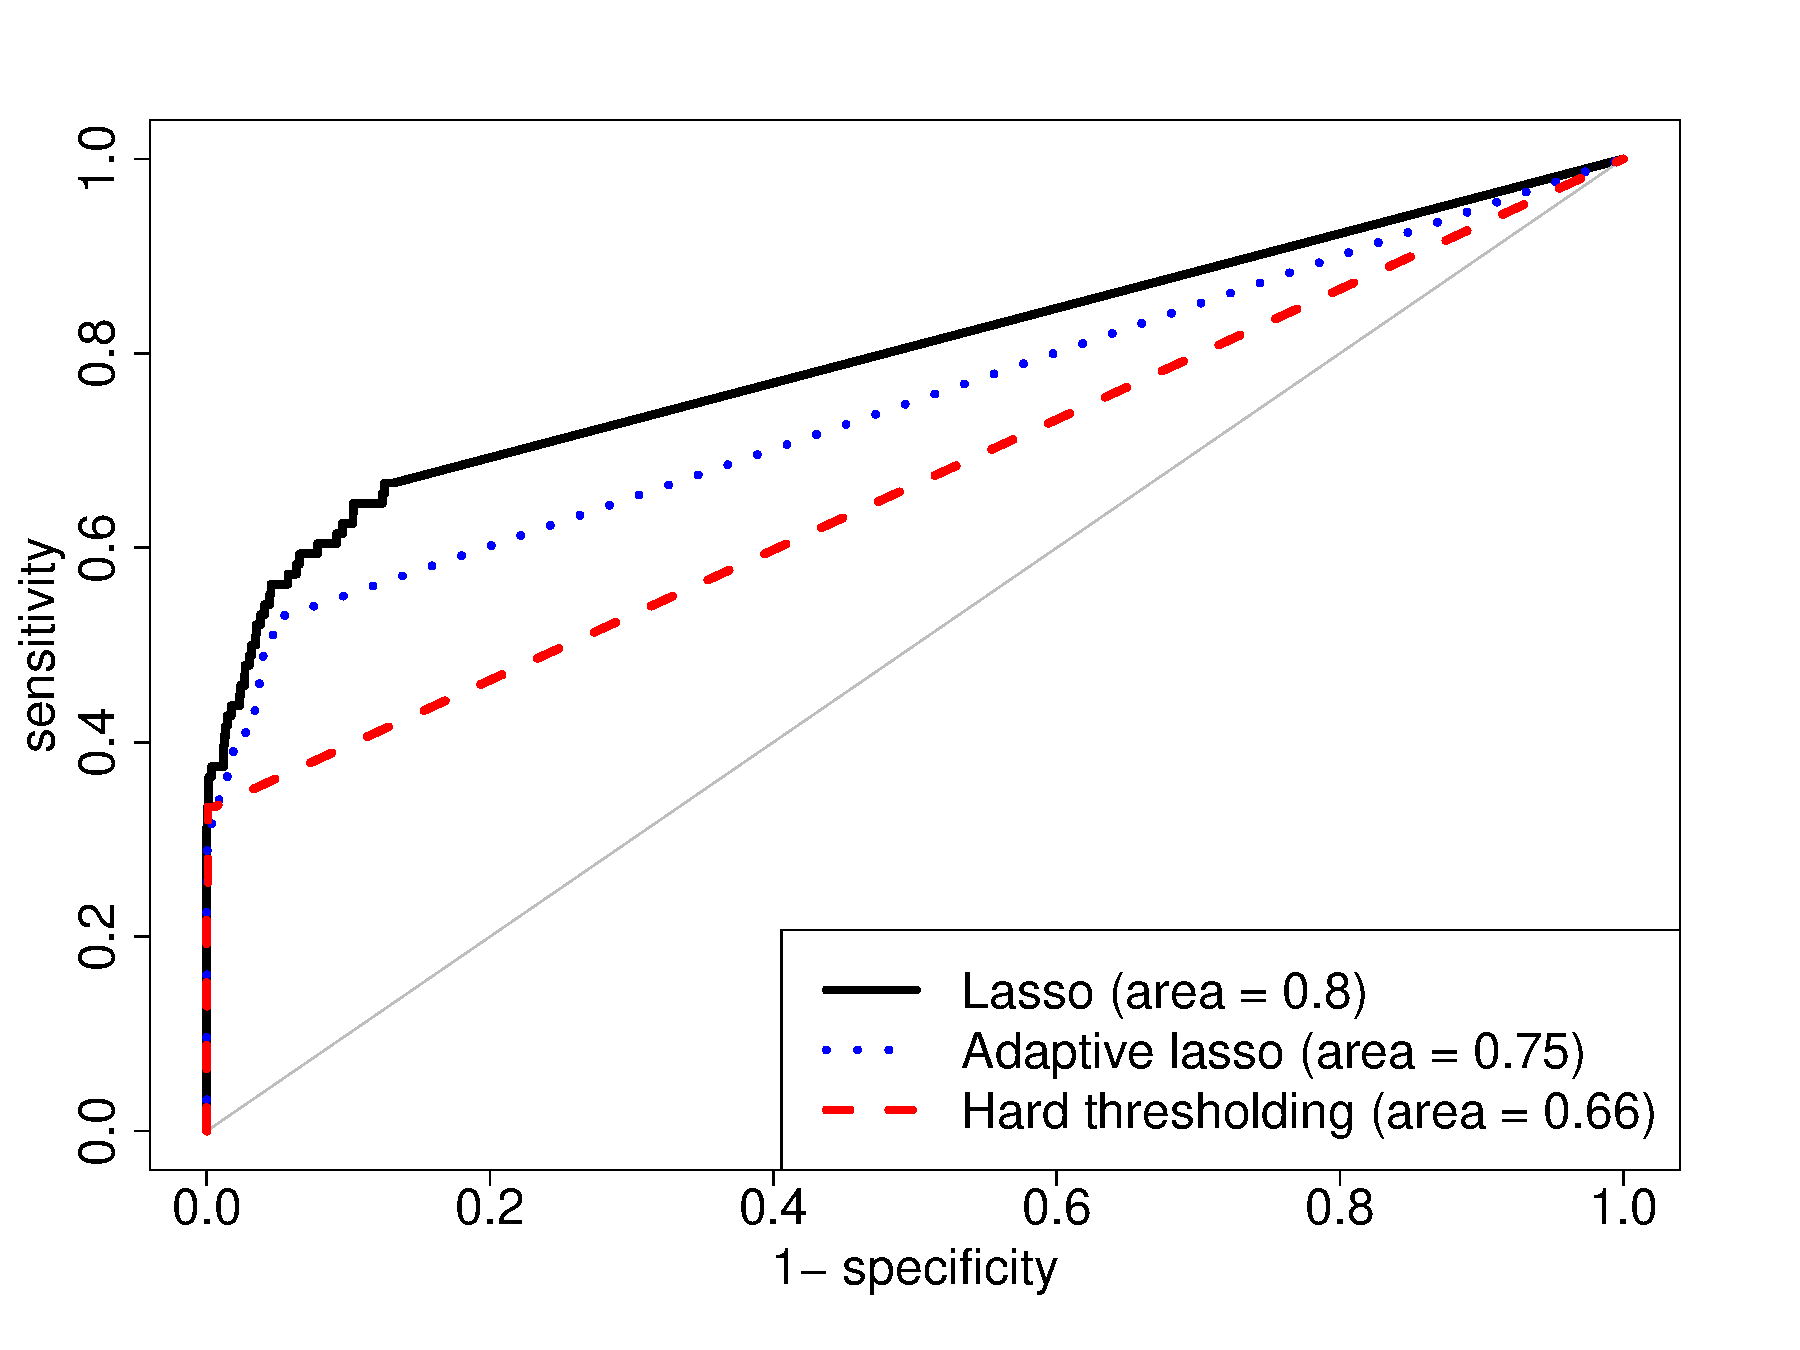
\includegraphics[width=0.48\textwidth]{img/ROC_100_96.pdf}
    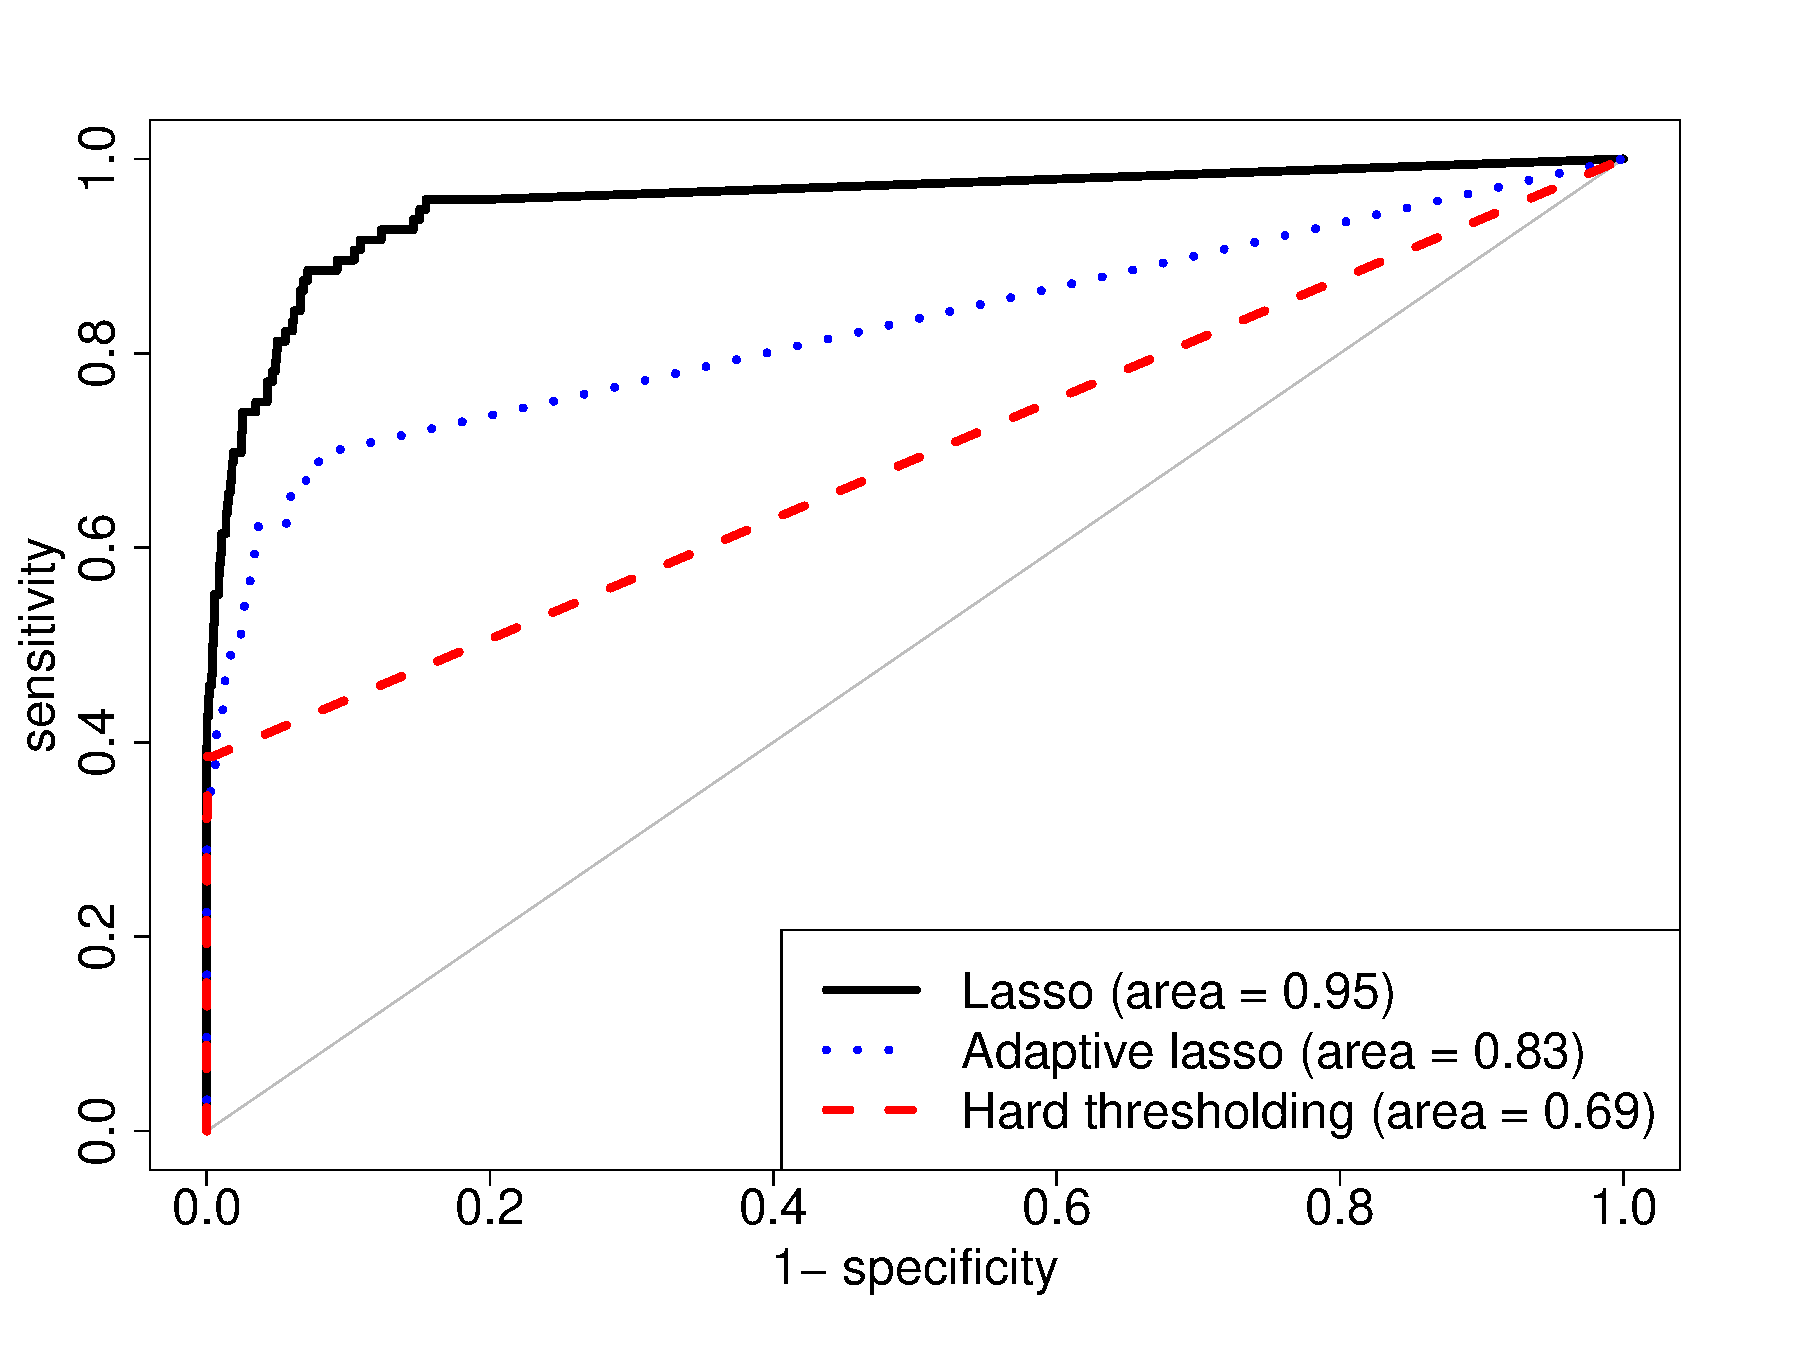
\includegraphics[width=0.48\textwidth]{img/ROC_200_96.pdf}
    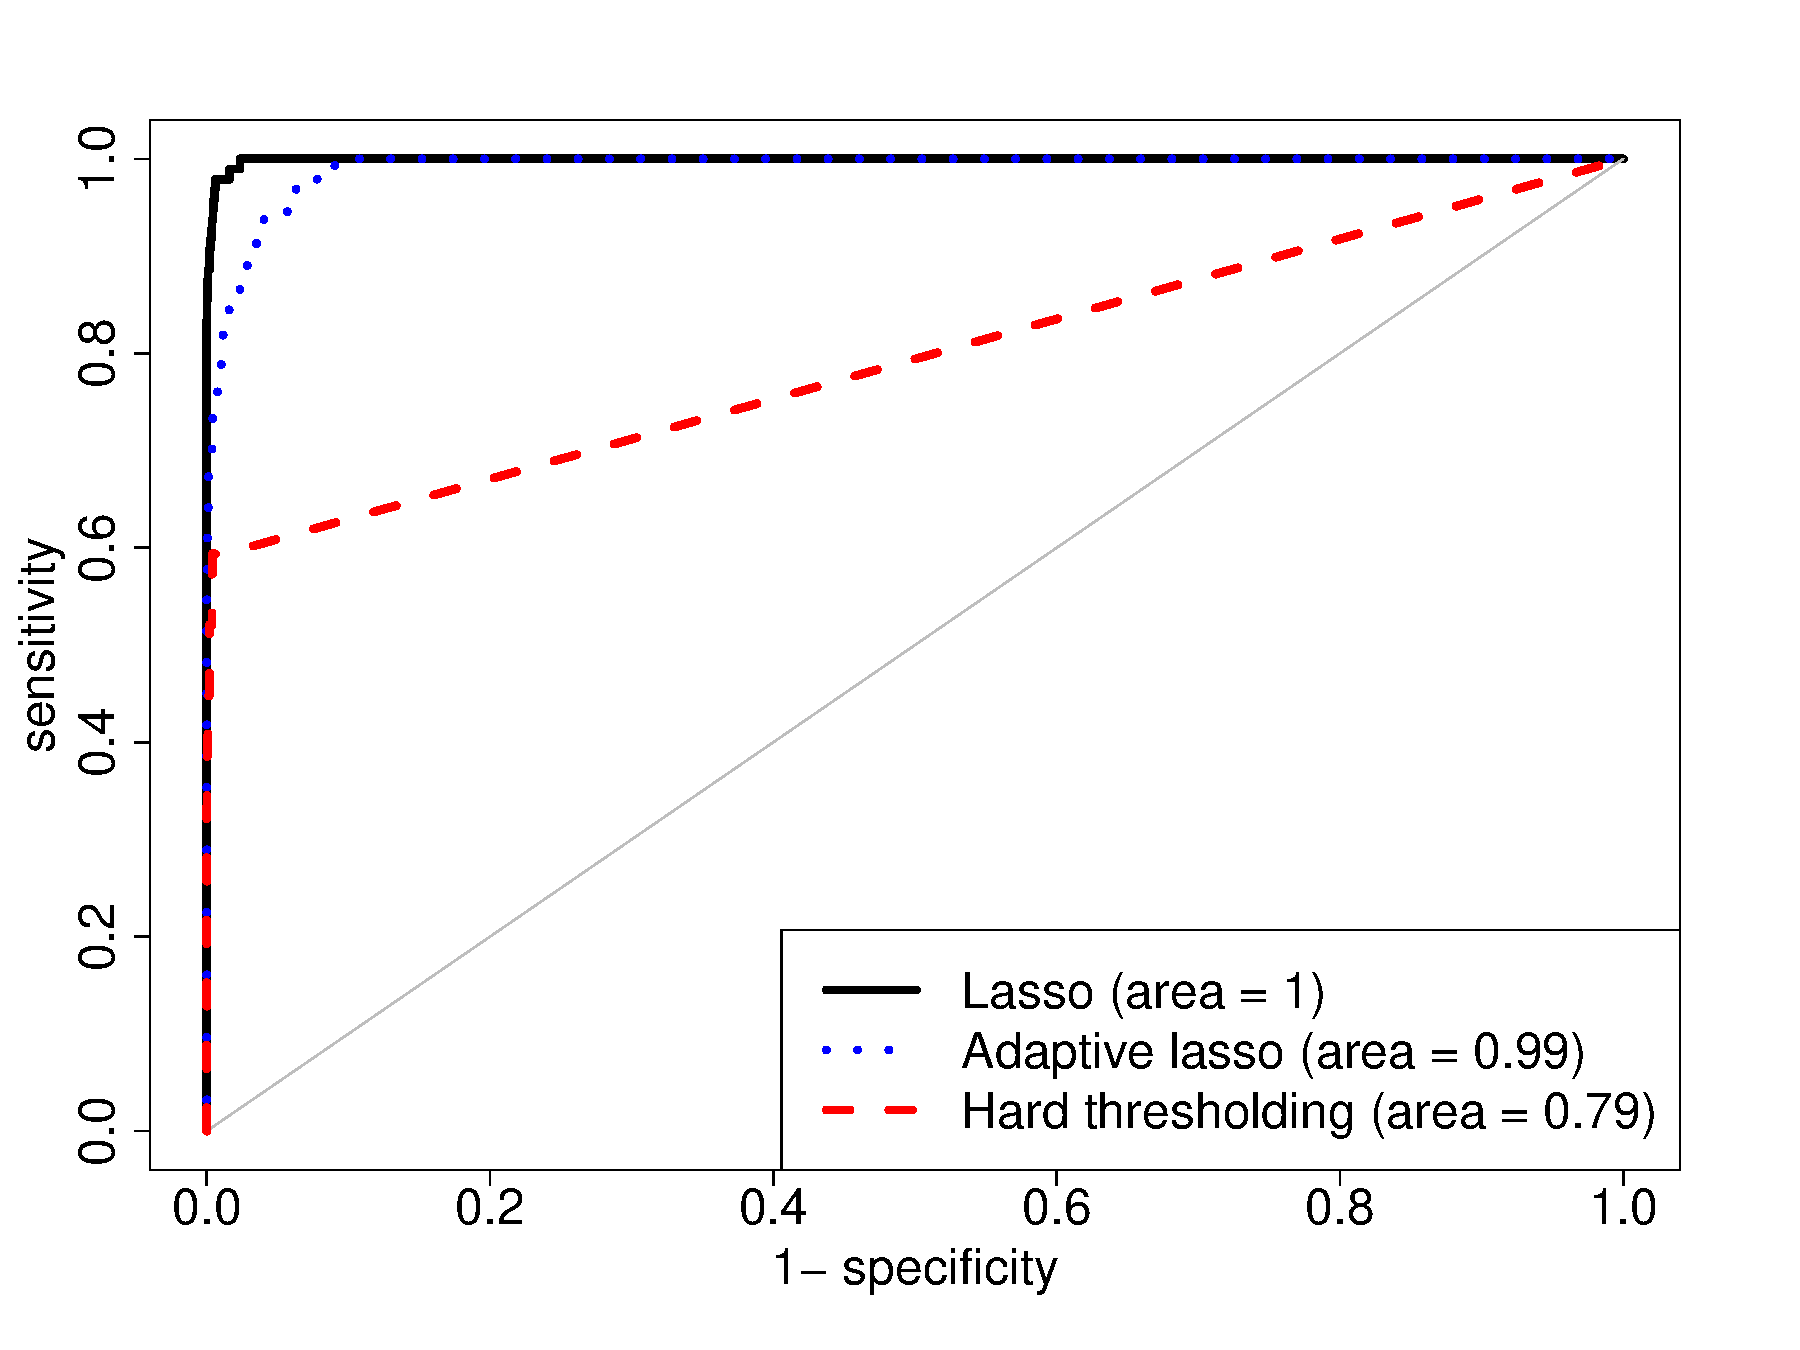
\includegraphics[width=0.48\textwidth]{img/ROC_400_96.pdf} 
    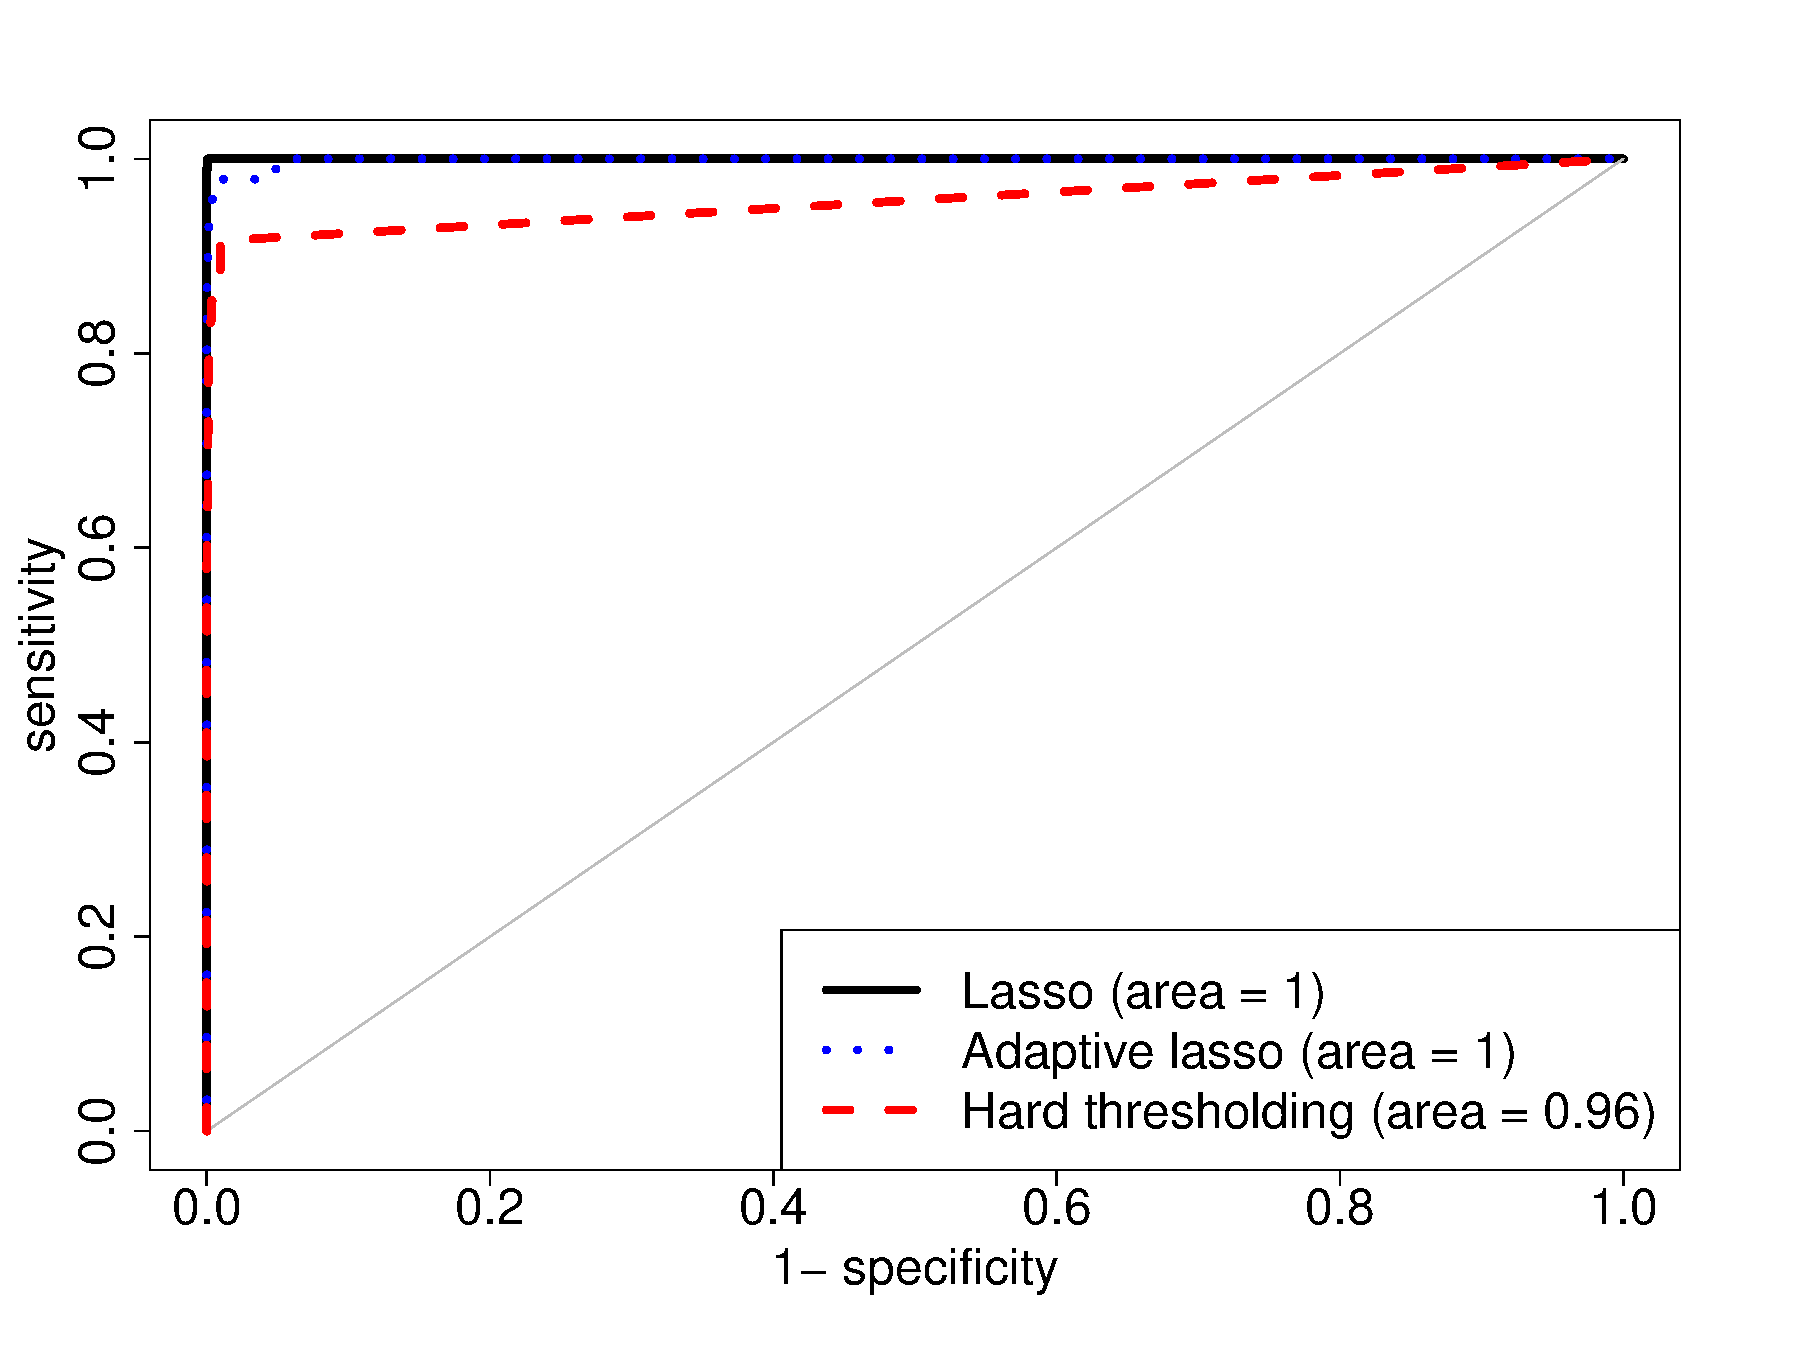
\includegraphics[width=0.48\textwidth]{img/ROC_600_96.pdf}    
    \caption{Receiver Operating Characeristic (ROC) curves of hard thresholding, lasso and adaptive lasso for recovering coherence network of a $p = 96$ dimensional VAR(1) model using $n = 100$ (top left), $n = 200$ (top right), $n = 400$ (bottom left) and $n = 600$ (bottom right) time series observations.}
    \label{fig:roc}
\end{figure}


% The results for heterogeneous settings are reported in Tables \ref{table:rmise-heterogeneous} and \ref{table:precision-heterogeneous}. Compared to homogeneous setting, RMISE of the three thresholding based methods outperform shrinkage estimators by a larger margin. {\color{red} [Sumanta: add description of precision/recall, and Figure \ref{fig::hetero}]. }




%\subsection{Tables and Graphs}




\section{Application: Sketching}
\label{appendix:sketching}
Beyond random projection, our novel TRP also has an important application in sketching. Sketching is an important technique to accelerate expensive computations with widespread applications, such as regression, low-rank approximation, and graph sparsification, etc. \citep{halko2011finding,woodruff2014sketching} 
% I have to think about how to argue tensor has a natural Khatri-Rao structure. 
The core idea behind sketching is to compress a large dataset, typically a matrix or tensor, into a smaller one by multiplying a random matrix. 
%Since the matrix multiplication is a linear operation, people can usually further extend sketching to distributed and online setting. 
In this section, we will mainly focus on the low-rank matrix approximation problem. Consider a matrix $\mathbf{X} \in \mathbb{R}^{m \times d}$ with rank $r$, 
we want to find the best rank-$r$ approximation with the minimal amount of time. The most common method is the randomized singular value decomposition (SVD), whose underlying idea is sketching. 


First, we compute the linear sketch $\mathbf{Z} \in \mathbb{R}^{m \times k}$ by $\mathbf{Z} =\mathbf{X}\mathbf{\Omega}$, where $\mathbf{\Omega} \in \mathbb{R}^{d \times r}$ is the random map. Then we compute the QR decomposition of $\mathbf{X}\mathbf{\Omega}$ by $\mathbf{Q}\mathbf{R} = \mathbf{Z}$, where $\mathbf{Q} \in \mathbb{R}^{m \times k}, \mathbf{R} \in \mathbb{R}^{r \times r}$. At the end, we project $\mathbf{X}$ onto the column space of $\mathbf{Q}$, and obtain the approximation $\hat{\mathbf{X}} = \mathbf{Q} \mathbf{Q}^\top \mathbf{X}$.  

With our TRP, we can significantly reduce the storage of the random map, while achieving similar rate of convergence as demonstrated in Figure \ref{fig:col_matrix}. 
With further variance reduction by taking the geometric-median over multiple runs, our TRP with variance reduction can achieve even better performance. The detailed implementation is given in Algorithm \ref{alg:var-red-structure-sketching}. And we will delay the theoretical analysis of this method for future works. 


\begin{algorithm}[H]
	\caption{Tensor Sketching with Variance Reduction}\label{alg:var-red-structure-sketching}
	\begin{algorithmic}[1]
		\Require $\mathbf{X} \in \mathbb{R}^{m \times d}$, where $d = \prod_{i=1}^N d_n$ and 
		\rm{RMAP} is a user-specified function that generates a random dimension reduction map. $T$ is the number of runs for variance reduction averaging. 
		\Function{SSVR}{$\mathbf{X}, \{d_n\}, k, T, \rm{RMAP}$}\\
		\text{For $t= 1 \dots T$}\\
		\text{For $i = 1 \dots N$} \\
		$\mathbf{\Omega}_i^{(t)} = \rm{RMAP}(d_i, k)$
		\State $\mathbf{\Omega}^{(t)} = \mathbf{\Omega}_1^{(t)} \odot \cdots \odot \mathbf{\Omega}_{N}^{(t)}$
		\State $(\mathbf{Q}^{(t)}, \sim ) = \rm{QR}(\mathbf{X}\mathbf{\Omega}^{(t)})$ 
		\State $\hat{\mathbf{X}}^{(t)} = \mathbf{Q}^{(t)}\mathbf{Q}^{(t)T}\mathbf{X}$
		\State
		$\hat{\mathbf{X}} = \frac{1}{T}\sum_{t=1}^T \hat{\mathbf{X}}^{(t)}$
		\State \Return $\mathbf{G}$
		\EndFunction
	\end{algorithmic}
\end{algorithm}

Furthermore, the extension of TRP to tensor data is also natural. To be specific, the $n^{th}$ unfolding of a large tensor $\mathscr{X} \in \mathbb{R}^{I_1 \times \cdots \times I_N}$, denoted as $\mathbf{X}^{(n)}$, has dimension $I_n \times I_{(-n)}$, where $I_{(-n)} = \prod_{i \neq n, i \in [N]} I_i$ . To construct a sketch for the unfolding, we need to create a random matrix of size $ I_{(-n)} \times k$. Then, our TRP becomes a natural choice to avoid the otherwise extremely expensive storage cost. For many popular tensor approximation algorithms, it is even necessary to perform sketching for every dimension of the tensor \citep{de2000multilinear,wang2015fast}. 
%such as Higher-Order Orthogonal Iteration \citep{de2000multilinear}, Fast CANDECOMP/PARAFAC decomposition \citep{wang2015fast}, our paper ? 
In the simulation section, we perform experiments for the unfolding of the higher-order order tensor with our structured sketching algorithms (Figure \ref{fig:col_matrix}). For more details in tensor algebra, please refer to \citep{kolda2009tensor}. 


\paragraph{Experimental Setup}
In sketching problems, considering a $N$-D tensor $\mathscr{X} \in \mathbb{R}^{I^N}$ with equal length along all dimensions, we want to compare the performance of the low rank approximation with different maps for its first unfolding $\mathbf{X}^{(1)} \in \mathbb{R}^{I \times I^{N-1}}$. 
	
We construct the tensor $\mathscr{X}$ in the following way. Generate a core tensor $\mathscr{C} \in \mathbb{R}^{r^N}$, with each entry $\rm{Unif}([0,1])$. Independently generate $N$ orthogonal arm matrices by first creating $\mathbf{A}_1, \dots, \mathbf{A}_N \in \mathbb{R}^{r \times I}$ and then computing the arm matrices by $(\mathbf{Q}_n, \sim) = \rm{QR}(\mathbf{A}_n)$, for $1 \leq n \leq N$.
\begin{equation}
\mathscr{X} = \mathscr{C} \times_1 \mathbf{Q}_1 \cdots \times_N \mathbf{Q}_N + \sqrt{\frac{0.01 \cdot \|\mathscr{X}^\natural\|_F^2}{I^N}} \mathcal{N}(0,1). \nonumber
\end{equation}
Then, we construct the mode-1 unfolding of $\mathbf{X} = \mathbf{X}^{(1)}$, which has a rank smaller than or equal to $r$. 

In our simulation, we consider the scenarios of 2-D ($900 \times 900$), 3-D ($400 \times 400 \times 400$), 4-D ($100 \times 100 \times 100 \times 100$) tensor data, with corresponding mode-1 unfolding of size $900 \times 900$, $400 \times 160000$, $100 \times 1000000$ respectively and $r = 5$. In each scenario, we compare the performance for Gaussian RP, TRP, and $\textup{TRP}_5$ maps with varying $k$ from 5 to 25. The TRP map in these scenarios has 2, 4, 6 components of size $30 \times k$, $20 \times k$, $10 \times k$ respectively. And the number of runs variance reduction averaging is $T = 5$. In the end, we evaluate the performance by generating the random matrix 100 times and compute the relative error $\frac{\|\mathbf{X} - \hat{\mathbf{X}}\|}{\|\mathbf{X}\|}$, and constructing a 95\% confidence interval for it.

\paragraph{Result}From Figure \ref{fig:col_matrix}, we can observe that the relative error decreases as $k$ increases as expected for all dimension reduction maps. The difference of the performance between the Khatri-Rao map and Gaussian map is small when $N = 2$, but increases when $N$ increases, whereas the Khatri-Rao variance reduced method is particularly effective producing strictly better performance than the other two. 

\begin{figure*}[ht!]
	\centering
	\begin{subfigure}{0.32\textwidth}
		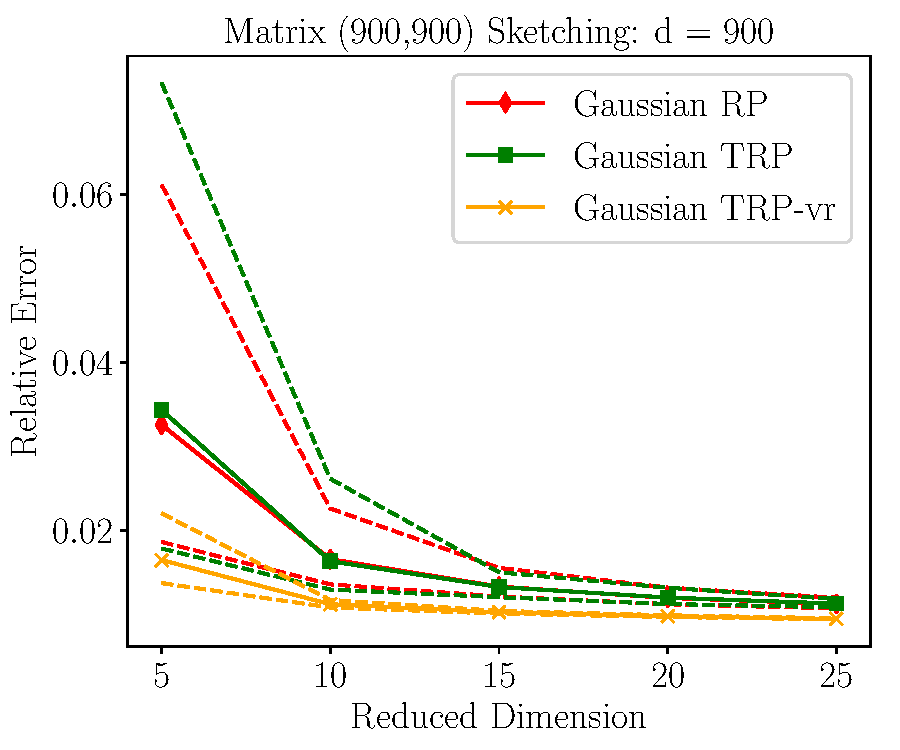
\includegraphics[scale = 0.3]{figure/col_dim2_krao_d900.pdf}
	\end{subfigure}
	\begin{subfigure}{0.32\textwidth}
		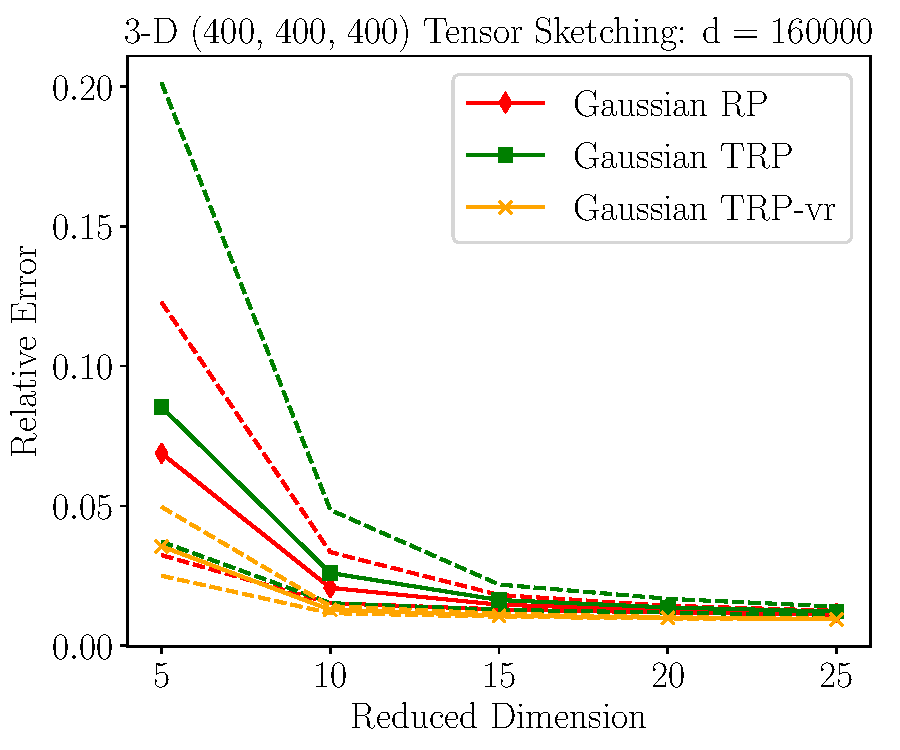
\includegraphics[scale = 0.3]{figure/col_dim3_krao_d160000.pdf}
	\end{subfigure}
	\begin{subfigure}{0.32\textwidth}
		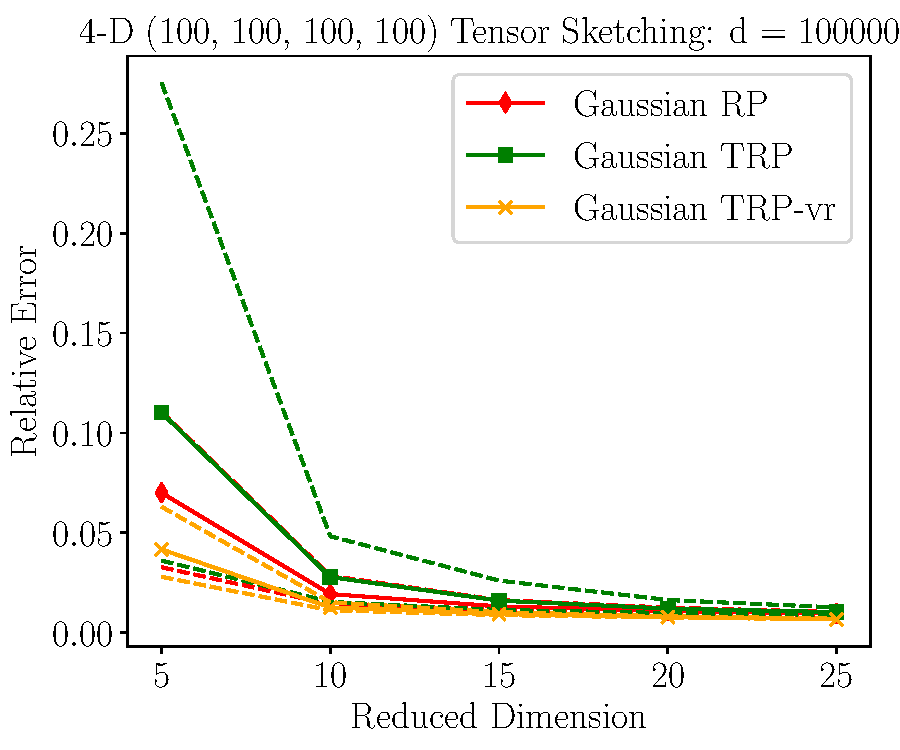
\includegraphics[scale = 0.3]{figure/col_dim4_krao_d1000000.pdf}
	\end{subfigure}\\
	\caption{Relative Error for the low-rank tensor unfolding approximation: \textit{we compare the relative errors for low-rank tensor approximation with different input size: 2-D ($900 \times 900$), 3-D ($400 \times 400 \times 400$), 4-D ($100 \times 100 \times 100 \times 100$). In each setting, we compare the performance of Gaussian RP, TRP, and $\textup{TRP}_5$. The dashed line stands for the 95\% confidence interval.}}
	\label{fig:col_matrix}
\end{figure*}


\section*{Conlusion}
We propose to do adaptive thresholding for weakly sparse spectral density estimation. In order to conquer some technical difficulty, we propose a new modified periodogram, which has the same  order in bias compared to the classic periodogram, while provides great convenience in theoretical development. Our adaptive thresholding relax the constraint in maximum operator norm  and achieve better convergence rate in theory. 
\clearpage
\bibliography{biblio.bib}
\bibliographystyle{plainnat}
\newpage
\begin{appendices}
\section{Proof for Bias and Variance Analysis}
\label{sec:appendix_proof}


Before presenting the proof for the main theory, we first define some new notations. Since these notations will only be used in technical proofs, we do not include them in the main body. 

\subsection*{Extra Notations for Technical Proofs} 
For a vector $\mathbf{x}$ with length $\prod_{n=1}^N d_n$, for simplicity, we introduce the multi-index for it: let $\mathbf{x}_{r_1, \cdots, r_N},\forall r_n \in [d_n]$, represent the $(1 + \sum_{n = 1}^N(r_n -1)s_n)^{th}$ element, where $s_n = \prod_{n+1}^Nd_n$ for $n < N$, and $1$ for $n = N$. For vector $\mathbf{r}_1$, $\mathbf{r}_2$, we say $\mathbf{r}_1 = \mathbf{r}_2$ if and only if 
all their elements are the same. 
\par 

Also, we let $\mathop{\mathbf{vec}}(\mathbf{A})$ be the vectorization operator for any matrix $\mathbf{A}\in \mathbb{R}^{d\times k}$, which stacks all columns of matrix $\mathbf{A}$ and returns a vector of length $kd$, 
$[\mathbf{A}(\cdot, 1); \cdots; \mathbf{A}(\cdot, k); ]$. Here we use semi-colon to denote the vertical stack of vectors $\mathbf{x}$ and $\mathbf{y}$ as $[\mathbf{x}; \mathbf{y}]$. As comparison, we use comma to mean stack row vector horizontally like $[\mathbf{x}^\top, \mathbf{y}^\top]$. 





\subsection*{Proof for Theorem \ref{thm: norm-preserve}}
\begin{proof}

We first give a sufficient condition for general random matrix to let  \eqref{eq:lemma-invariant-length-statement} be held, then we show that Khatri-Rao map with condition in Theorem \ref{thm: norm-preserve} satisfies these two general sufficient conditions. \par 



Consider a general random matrix $\mathbf{A}\in \mathbb{R}^{k \times d}$ and $\mathbf{x} \in \mathbb{R}^d$.
we claim if ~$\mathbb{E}{\mathbf{A}^2(r,s)}=1, \forall r,s $ and $\mathbb{E}{\mathbf{A}(r,s_1)\mathbf{A}(r,s_2)} = 0, \forall r \in[k], s_1\neq s_2 \in[d]$,
then $\mathbb{E}\| \frac{1}{\sqrt{k}}\mathbf{y}\|_2^2 = \|\mathbf{x}\|_2^2$, when $\mathbf{y}=\mathbf{A}\mathbf{x}$. To see why, it suffices to show that $\mathbb{E} y_r^2 = \|x\|^2_2$.
\begin{equation} \label{eq:row-length}
\begin{aligned}
&\mathbb{E}{y_r^2} = \mathbb{E}{\sum_{s_1=1}^d\sum_{s_2=1}^d \mathbf{A}(r,s_1)\mathbf{A}(r,s_2)x_{s_1}x_{s_2}} \\
&= \sum_{s=1}^d \mathbf{A}^2(r,s)x_s^2 = \|\mathbf{x}\|^2_2,  \nonumber
\end{aligned}
\end{equation}
where the first equation in the second line comes from the fact that $\mathbb{E} {\mathbf{A}(r,s_1)\mathbf{A}(r,s_2)}  = 0$ for $s_1\neq s_2$ and the second equation in the second line comes from that $\mathbb{E}{\mathbf{A}^2(r,s)} =1$.

Then, we will prove Theorem \ref{thm: norm-preserve} by induction. 
We first show that for two matrices $\mathbf{B}_1 \in \mathbb{R}^{d_1\times k}, \mathbf{B}_2 \in \mathbb{R}^{d_2\times k}$ whose entries satisfy the two conditions in Theorem \ref{thm: norm-preserve}: $\mathbb{E} \mathbf{B}^2_{n}(r,s)=1$
and  $\mathbb{E} [ \mathbf{B}_{n}(r_1,s)\mathbf{B}_{n}(r_2,s)] =0$ for $n=1,2, s\in [d], r, r_1\neq r_2\in [d_n]$, we have $\mathbf{A} = (\mathbf{B}_1 \odot\mathbf{B}_2 )^\top $ satifies the two sufficient conditions stated previously. It suffices to restrict our focus to the first row of $\mathbf{\Omega}$ and we apply the multi-index to it. For any $1\le r_1\le d_1, 1\le r_2\le d_2$, 
\begin{equation}
\begin{aligned}
&\mathbb{E}  \mathbf{A}^2_{1}(k_1,k_2) = \mathbb{E} \mathbf{B}^2_{1}(k_1,1)\mathbf{B}^2_{2}(k_2,1)\\
& =  \mathbb{E} \mathbf{B}^2_{1}(k_1,1) \mathbb{E} \mathbf{B}^2_{2}(k_1,1) = 1.  ~(\text{independence bewteen} ~ \mathbf{B}_i, i=1,2 )
\nonumber
\end{aligned}
\end{equation}
To avoid confusion in notation, we argue that $ \mathbf{A}(1,\cdot)$ is the first row vector of $ \mathbf{A}$ of size $d_1d_2$, and we apply the multi-index to it.  Also, for two different elements in the first row of $\mathbf{A}$: $ \mathbf{A}_{1}(k_1,k_2) \mathbf{A}_{1}(s_1,s_2)$ at least one of $k_1\neq s_1$, $k_2\neq s_2$ hold. Without losing generality, assuming $k_1\neq s_1$, 

\begin{equation}
\begin{aligned}
&\mathbb{E}  \mathbf{A}_{1}(k_1,k_2) \mathbf{A}_{1}(s_1,s_2)  = \mathbb{E} \mathbf{B}_{1}(k_1,1)\mathbf{B}_{2}(k_2,1)\mathbf{B}_{1}(s_1,1)\mathbf{B}_{2}(s_2,1)\\
& =  \mathbb{E} \mathbb{E}\left[ \mathbf{B}_{1}(k_1,1)\mathbf{B}_{1}(k_2,1)\mathbf{B}_{2}(k_2,1)\mathbf{B}_{2}(s_2,1)  \mid  \mathbf{B}_{2}(k_2,1)\mathbf{B}_{2}(s_2,1)\right]\\
& =  \mathbb{E}  \mathbf{B}_{2}(k_2,1)\mathbf{B}_{2}(s_2,1) \mathbb{E}\left[ \mathbf{B}_{1}(k_1,1)\mathbf{B}_{1}(s_1,1) \right]  = 0,
\nonumber
\end{aligned}
\end{equation}
where we use the fact that entries within/across $B_i$ are independent with each other and have zero expectation. \par 

Notice that two conditions for $\mathbf{A}  =  (\mathbf{B}_1 \odot\mathbf{B}_2 )^\top$ directly show that $\mathbf{B}_1 \odot\mathbf{B}_2$ satisfies two conditions in Theorem \ref{thm: norm-preserve}, we could use a standard mathematical induction argument to finish the proof for $\textup{TRP}$. For TRP(T), 
\begin{equation}
\begin{aligned}
&\mathbb{E}\|\textup{TRP}_T(\mathbf{x})\|^2_2=\frac{1}{T} \mathbb{E}\|\sum_{t=1}^T \textup{TRP}^{(t)}(\mathbf{x})\|^2_2\\
&= \frac{1}{T}\sum_{t=1}^T\mathbb{E} \|\textup{TRP}^{(t)}(\mathbf{x})\|^2_2= \|\mathbf{x}\|^2_2,
\nonumber 
\end{aligned}
\end{equation}
where in the second line we use the fact that each $\textup{TRP}^{(t)}$ is independent with each other.
\end{proof}


Next we introduce a lemma which shows that by bounding the deviation for the norm square of each vector, we could also bound the deviation for inner product. Although it is commonly known in any random projection literature, for completeness, we still list the lemma with proof here. 




\subsection*{Proof for Theorem \ref{thm:variance}}
\begin{proof}
Let $\mathbf{y}=\mathbf{Ax}$. We know from Theorem \ref{thm: norm-preserve} that $\mathbb{E}\|\textup{TRP}(\mathbf{x})\|^2_2 = \frac{1}{k}\mathbb{E}\|\mathbf{Ax}\|^2= \|\mathbf{x}\|^2_2$. 
Notice 
\[
\mathbb{E}(\|\textup{TRP}_T(\mathbf{x})\|^2_2) = \|\mathbf{x}\|^2_2, 
\]
and $\mathbb{E} y_1^2=\|x\|_2^2$ as shown in the poof of Lemma \ref{thm: norm-preserve}. It is easy to see that
\[
\mathbb{E}\|\mathbf{y}\|^4_2 = \sum_{i=1}^k \mathbb{E} y_i^4 + \sum_{i\neq j} \mathbb{E} y_i^2y_j^2.
\]
Again, as shown in Theorem \ref{thm: norm-preserve}, $\mathbb{E} y_i^2y_j^2 =\mathbb{E} y_i^2 \mathbb{E} y_j^2 = \|\mathbf{x}\|^4$. To find $\mathbb{E}\|\mathbf{y}\|^4_2$, it suffices to find $\mathbb{E} y_1^4$ by noticing that $y_i$ are iid random variables. Let $\Omega$ be the set containing all corresponding multi-index vector for $\{1,\cdots, \prod_{n=1}^N d_n\}$. 
\begin{equation}
\begin{aligned}
&y_1^4 = \left[\sum_{\mathbf{r}\in \Omega} \mathbf{A}(1,\mathbf{r}) x_{\mathbf{r}}\right]^4 = \sum_{\mathbf{r}\in \Omega} \mathbf{A}^4(1,\mathbf{r}) x^4_{\mathbf{r}} + 3\sum_{\mathbf{r}_1 \neq \mathbf{r}_2 \in \Omega} \mathbf{A}^2(1,\mathbf{r}_1) x^2_{\mathbf{r}_1}\mathbf{A}^2(1,\mathbf{r}_2) x^2_{\mathbf{r}_2}\\
&+6\sum_{\mathbf{r}_1 \neq \mathbf{r}_2 \neq \mathbf{r}_3 \in \Omega} \mathbf{A}^2(1,\mathbf{r}_1) x_\mathbf{\mathbf{r}_1} \mathbf{A}(1,\mathbf{r}_2)x_{\mathbf{r}_2}\mathbf{A}(1,\mathbf{r}_3)x_{\mathbf{r_3}}+4\sum_{\mathbf{r}_1 \neq \mathbf{r}_2 \in \Omega} \mathbf{A}^3(1,\mathbf{r}_1) x^3_{\mathbf{r}_1}\mathbf{A}(1,\mathbf{r}_2) x_{\mathbf{r}_2}\\
&+\sum_{\mathbf{r}_1 \neq \mathbf{r}_2 \neq \mathbf{r}_3\neq \mathbf{r}_4 \in \Omega} \mathbf{A}(1,\mathbf{r}_1) x_{\mathbf{r}_1}\mathbf{A}(1,\mathbf{r}_2) x_{\mathbf{r}_2}\mathbf{A}(1,\mathbf{r}_3) x_{\mathbf{r}_3}\mathbf{A}(1,\mathbf{r}_4) x_{\mathbf{r}_4}.\nonumber
\end{aligned}
\end{equation}
It is not hard to see that except for the first line, the expectation of second and third line is zero. 
\[
\mathbb{E} \mathbf{A}^4(1,\mathbf{r}) = \mathbb{E} \mathbf{A}^4_1 (1, r_1) \cdots \mathbf{A}^4_N(1, r_N) = \Delta^N. 
\]
Also with proof in Theorem \ref{thm: norm-preserve}, 
\[
\mathbb{E} \mathbf{A}^2(1,\mathbf{r}_1)\mathbf{A}^2(1,\mathbf{r}_2) = \mathbb{E} \mathbf{A}^2(1,\mathbf{r}_1) \mathbb{E}  \mathbf{A}^2(1,\mathbf{r}_2)  = 1.
\]
Combining these two together, we have 
\begin{equation} \label{eq:TRP_fourth_moment}
\begin{aligned}
&\mathbb{E}\|\textup{TRP}(\mathbf{x})\|^4 = \frac{1}{k^2}\left[k(\Delta^N-3)\|\mathbf{x}\|_4^4 +3k\|\mathbf{x}\|_2^4  +(k-1)k \|\mathbf{x}\|_2^4\right]\\
& =  \frac{1}{k}\left[(\Delta^N-3)\|\mathbf{x}\|_4^4 +2\|\mathbf{x}\|_2^4\right]+\|\mathbf{x}\|_2^4.  
\end{aligned}
\end{equation}
Therefore, 
\[
\textrm{Var}(\|\textup{TRP}(\mathbf{x})\|^2_2) = \mathbb{E}\|\textup{TRP}(\mathbf{x})\|^4_2 -  (\mathbb{E}\|\textup{TRP}(\mathbf{x})\|^2_2)^2 = \frac{1}{k}\left[(\Delta^N-3)\|\mathbf{x}\|_4^4 +2\|\mathbf{x}\|_2^4\right].
\]
Now we switch to see how much variance could be reduced by the variance reduction method. With Theorem \ref{thm: norm-preserve}, we already know that $\mathbb{E} \|\textup{TRP}_T(\mathbf{x})\|^2_2= \|\mathbf{x}\|_2^2$. The rest is to calculate $\mathbb{E} \|\textup{TRP}_T(\mathbf{x})\|^4_2$ out.
\begin{equation}
\begin{aligned}
&\|\textup{TRP}_T(\mathbf{x})\|^4_2 = \frac{1}{T^2}\left[\sum_{t=1}^T \|\textup{TRP}^{(t)}(\mathbf{x})\|^2_2+\sum_{t_1 \neq t_2} \langle \textup{TRP}^{(t_1)}(\mathbf{x}), \textup{TRP}^{(t_2)}(\mathbf{x}) \rangle \right]^2\\
&= \frac{1}{T^2} \left[ \sum_{t=1}^T \|\textup{TRP}^{(t)}(\mathbf{x})\|^4_2+\sum_{t_1\neq t_2}\|\textup{TRP}^{(t_1)}(\mathbf{x})\|^2_2\|\textup{TRP}^{(t_2)}(\mathbf{x})\|^2_2 +2\sum_{t_1\neq t_2}\langle \textup{TRP}^{(t_1)}(\mathbf{x}), \textup{TRP}^{(t_2)}(\mathbf{x}) \rangle^2 +\text{rest} \right].\nonumber 
\end{aligned}
\end{equation}
It is not hard to show that $\mathbb{E}(\text{rest}) = 0$. Following the definition of $\mathbf{y}$, 

\begin{equation}
\mathbb{E} \|\textup{TRP}^{(t_1)}(\mathbf{x})\|^2_2\|\textup{TRP}^{(t_2)}(\mathbf{x})\|^2_2= \|\mathbf{x}\|_2^4, \nonumber 
\end{equation}
and 
\begin{equation} 
\begin{aligned}
&\mathbb{E} \langle \textup{TRP}^{(t_1)}(\mathbf{x}), \textup{TRP}^{(t_2)}(\mathbf{x}) \rangle^2\\ 
&=\frac{1}{k^2} \mathbb{E} \left[ \sum_{i=1}^k y^{(t_1)}_i y^{(t_2)}_i \right]^2 \\
&= \frac{1}{k}  \mathbb{E} (y^{(t_1)}_1)^2\mathbb{E} (y^{(t_2)}_1)^2 = \frac{1}{k}\|\mathbf{x}\|_2^4. \nonumber
\end{aligned}
\end{equation}
Combining all these together, we could show that 
\begin{equation}
\begin{aligned}
\textrm{Var}(\|\textup{TRP}_T(\mathbf{x})\|_2^2) &= \mathbb{E}\|\textup{TRP}_T(\mathbf{x})\|^4_2 -  (\mathbb{E}\|\textup{TRP}_T(\mathbf{x})\|^2_2)^2\\ 
&= \frac{1}{T^2} \left[ \frac{T}{k}\left[(\Delta^N-3)\|\mathbf{x}\|_4^4 +2\|\mathbf{x}\|_2^4 \right]\right.\\
&\left. + T\|\mathbf{x}\|_2^4 +T(T-1)\|\mathbf{x}\|_2^4+\frac{2T(T-1)}{k}\|\mathbf{x}\|_2^4 \right] - \|\mathbf{x}\|_2^4 \\ 
&= \frac{1}{Tk}(\Delta^N-3)\|\mathbf{x}\|_4^4 + \frac{2}{k}\|\mathbf{x}\|_2^4. \nonumber
\end{aligned}
\end{equation}
\end{proof}

\subsection*{Proof for Lemma \ref{lem:inner_product_TRP}} 
\begin{proof}
First, we show the unbiasedness of the inner product estimation: 

\begin{equation} \label{eq: inner_prod_unbias}
\begin{aligned}
\mathbb{E}(\langle \textup{TRP}(\mathbf{x}),\textup{TRP}(
\mathbf{y})\rangle) = [ \| \textup{TRP}(\mathbf{x}) + \textup{TRP}(\mathbf{y})\|_2^2 - \| \textup{TRP}(\mathbf{x})\|_2^2 -  \| \textup{TRP}(\mathbf{y})\|_2^2  ]/2  = \langle \mathbf{x}, \mathbf{y} \rangle.
\nonumber
\end{aligned} 
\end{equation}


The equation above follows from Thm \ref{thm: norm-preserve}, the unbiasedness of norm estimation. We can apply the similar idea to get $\mathbb{E}(\langle \textup{TRP}_T(\mathbf{x}),\textup{TRP}_T(
\mathbf{y})\rangle) = \langle \mathbf{x}, \mathbf{y}\rangle$. 

Now, let $\mathbf{u} = \mathbf{A}\mathbf{x}$, $\mathbf{v} = \mathbf{A}\mathbf{y}$. Then, 

\begin{equation*}
\begin{aligned}
(u_1 v_1)^2 &= [\sum_{\mathbf{r} \in \Omega} \mathbf{A}(1,\mathbf{r}) x_\mathbf{r}]^2 [\sum_{\mathbf{r} \in \Omega} \mathbf{A}(1,\mathbf{r}) 
y_\mathbf{r}]^2 \\  
&= \sum_{\mathbf{r}} \mathbf{A}(1,\mathbf{r})^4 x_{\mathbf{r}}^2 y_{\mathbf{r}}^2 +
 \sum_{\mathbf{r}_1 \neq \mathbf{r}_2} \mathbf{A}(1, \mathbf{r}_1)^2 \mathbf{A}(1, \mathbf{r}_2)^2 x_{\mathbf{r}_1}^2 y_{\mathbf{r}_2}^2 \\
&+ 2\sum_{\mathbf{r}_1 \neq \mathbf{r}_2 } \mathbf{A}(1, \mathbf{r}_1)^2 \mathbf{A}(1, \mathbf{r}_2)^2 x_{\mathbf{r}_1} x_{\mathbf{r}_2} y_{\mathbf{r}_1} y_{\mathbf{r}_2} + \text{rest} .,\\
\end{aligned}
\end{equation*} 

Since $\mathbb{E} \mathbf{A}(1,\mathbf{r}) = 0, \; \forall \mathbf{r}$, $\mathbb{E}(\text{rest}) = 0$. Also with proof in Thm \ref{thm: norm-preserve}, 
\[
\mathbb{E} \mathbf{A}^2(1,\mathbf{r}_1)\mathbf{A}^2(1,\mathbf{r}_2) = \mathbb{E} \mathbf{A}^2(1,\mathbf{r}_1) \mathbb{E}  \mathbf{A}^2(1,\mathbf{r}_2)  = 1.
\]
And, 
\[
\mathbb{E} \mathbf{A}^4(1,\mathbf{r}) = \mathbb{E} \mathbf{A}^4_1 (1, r_1) \cdots \mathbf{A}^4_N(1, r_N) = \Delta^N. 
\]

Then, similar to \eqref{eq:TRP_fourth_moment}, we can obtain:  
\begin{equation}\label{eq:inner_prod_second_moment}
\begin{aligned}
\mathbb{E}(\langle \textup{TRP}(\mathbf{x}), \textup{TRP}(\mathbf{y}) \rangle)^2 &= \frac{1}{k^2}\mathbb{E}[ \sum_{i,j} u_iv_iu_jv_j]^2 
= \frac{1}{k^2}\mathbb{E}[ \sum_{i} (u_iv_i)^2]  + 
\frac{1}{k^2} \mathbb{E}[\sum_{i \neq j}(u_i v_i u_j v_j)]  \\
&= \frac{1}{k} \mathbb{E}(u_1v_1)^2 + \frac{k(k-1)}{k^2} \langle \mathbf{x}, \mathbf{y}\rangle^2\\ 
&= \frac{1}{k} [ (\Delta^N - 3) \sum_{\mathbf{r}}x_{\mathbf{r}}^2y_{\mathbf{r}}^2  + \|\mathbf{x}\|_2^2\|\mathbf{y}\|^2_2 + \langle \mathbf{x}, \mathbf{y} \rangle^2 ] + \langle \mathbf{x}, \mathbf{y}\rangle^2.
\end{aligned} 
\end{equation} 

Then, with the unbiasedness of TRP map, we get
\begin{equation}
\begin{aligned}
\textrm{Var}(\langle \textup{TRP}(\mathbf{x}) , \textup{TRP}(\mathbf{y}) \rangle) &= \mathbb{E}(\langle \textup{TRP}(\mathbf{x}), \textup{TRP}(\mathbf{y}) \rangle^2) - (\mathbb{E}\langle \textup{TRP}(\mathbf{x}), \textup{TRP}(\mathbf{y}) \rangle)^2 \\
&= \frac{1}{k} [ (\Delta^N - 3) \sum_{\mathbf{r}}x_{\mathbf{r}}^2y_{\mathbf{r}}^2  + \|\mathbf{x}\|_2^2\|\mathbf{y}\|^2_2 + \langle \mathbf{x}, \mathbf{y} \rangle^2].
\nonumber
\end{aligned}
\end{equation} 

Now, we proceed to find the variance for the inner product estimation with $\textup{TRP}_T$. Since $\var(\langle \textup{TRP}_T(\mathbf{x}), \textup{TRP}_T(\mathbf{y}) \rangle) = 
\mathbb{E}(\langle \textup{TRP}_T(\mathbf{x}), \textup{TRP}_T(\mathbf{y}) \rangle^2) - (\mathbb{E}\langle \textup{TRP}_T(\mathbf{x}), \textup{TRP}_T(\mathbf{y}) \rangle)^2$, we first compute: 
\begin{equation} 
\begin{aligned}
\langle \textup{TRP}_T(\mathbf{x}), \textup{TRP}_T(\mathbf{y}) \rangle^2 &= \frac{1}{T^2} \langle \sum_{i = 1}^T \textup{TRP}^{(i)}(\mathbf{x}),  \sum_{j = 1}^T \textup{TRP}^{(j)}(\mathbf{y}) \rangle^2\\
&= \frac{1}{T^2} \sum_{i =1}^T \langle  \textup{TRP}^{(i)}(\mathbf{x}), \textup{TRP}^{(i)}(\mathbf{y}) \rangle^2 \\
&+ \frac{1}{T^2}\sum_{i \neq j}(\langle  \textup{TRP}^{(i)}(\mathbf{x}), \textup{TRP}^{(i)}(\mathbf{y}) \rangle)(\langle  \textup{TRP}^{(j)}(\mathbf{x}), \textup{TRP}^{(j)}(\mathbf{y}) \rangle) \\
&+ \frac{2}{T^2}\sum_{i \neq j} \langle  \textup{TRP}^{(i)}(\mathbf{x}), \textup{TRP}^{(j)}(\mathbf{y}) \rangle^2 + \text{rest}.  \nonumber
\end{aligned} 
\end{equation}

Following the definition of the TRP map, we can see:
\begin{equation}
\begin{aligned}
&\mathbb{E} \langle \textup{TRP}^{(t_1)}(\mathbf{x}), \textup{TRP}^{(t_2)}(\mathbf{y}) \rangle^2\\ 
&=\frac{1}{k^2} \mathbb{E} \left[ \sum_{i=1}^k u^{(t_1)}_i v^{(t_2)}_i \right]\left[ \sum_{i=1}^k u^{(t_1)}_i v^{(t_2)}_i \right] \\
&= \frac{1}{k}  \mathbb{E} [u^{(t_1)}_1 u^{(t_1)}_1]\mathbb{E} [v^{(t_2)}_1 v^{(t_2)}_1] = \frac{1}{k}\|\mathbf{x}\|_2^2\|\mathbf{y}\|_2^2. \nonumber
\end{aligned}
\end{equation}


First, $\mathbb{E}(\text{rest}) = 0$. Then, combining all the above results, we obtain:
\begin{equation*}
\begin{aligned}
\var(\langle \textup{TRP}_T(\mathbf{x}), \textup{TRP}_T(\mathbf{y}) \rangle) &= 
\mathbb{E}(\langle \textup{TRP}_T(\mathbf{x}), \textup{TRP}_T(\mathbf{y}) \rangle^2) - (\mathbb{E}\langle \textup{TRP}_T(\mathbf{x}), \textup{TRP}_T(\mathbf{y}) \rangle)^2 \\   
&= 
\mathbb{E}(\langle \frac{1}{T^2}\sum_{i} \textup{TRP}^{(i)}(\mathbf{x}), \frac{1}{T^2} \sum_{j} \textup{TRP}^{(j)}(\mathbf{y}) \rangle^2) - (\mathbb{E}\langle \textup{TRP}_T(\mathbf{x}), \textup{TRP}_T(\mathbf{y}) \rangle)^2 \\  
&= \frac{1}{T^2}\mathbb{E}(\sum_{i} \langle \textup{TRP}^{(i)}(\mathbf{x}), \textup{TRP}^{(i)}(\mathbf{y}) \rangle^2 \\
&+ \sum_{i \neq j} \langle \textup{TRP}^{(i)}(\mathbf{x}), \textup{TRP}^{(i)}(\mathbf{y}) \rangle \langle \textup{TRP}^{(j)}(\mathbf{x}), \textup{TRP}^{(j)}(\mathbf{y}) \rangle \\
&+2 \sum_{i \neq j} \langle \textup{TRP}^{(i)}(\mathbf{x}), \textup{TRP}^{(j)}(\mathbf{y}) \rangle^2 ) - (\mathbb{E}\langle \textup{TRP}_T(\mathbf{x}), \textup{TRP}_T(\mathbf{y}) \rangle)^2 \\   
&=  \frac{1}{T^2}\left[ \frac{T}{k} [ (\Delta^N - 3) \sum_{\mathbf{r}}x_{\mathbf{r}}^2y_{\mathbf{r}}^2  + \|\mathbf{x}\|_2^2\|\mathbf{y}\|^2_2 + \langle \mathbf{x}, \mathbf{y} \rangle^2 ] + T\langle \mathbf{x}, \mathbf{y} \rangle^2 \right.\\
&\left. +  \frac{2T(T-1)}{k} \|\mathbf{x}\|_2^2\|\mathbf{y}\|_2^2 + T(T-1)\langle \mathbf{x}, \mathbf{y}\rangle^2 \right] - \langle \mathbf{x}, \mathbf{y} \rangle^2 \\  
&= \frac{1}{kT}(\Delta^N -3) \sum_{\mathbf{r}}x_{\mathbf{r}}^2y_{\mathbf{r}}^2 +  (\frac{2}{k} - \frac{1}{kT})\|\mathbf{x}\|_2^2\|\mathbf{y}\|_2^2 + \frac{1}{kT}\langle \mathbf{x}, \mathbf{y} \rangle^2.  \\
\end{aligned}  
\end{equation*}

\end{proof}
\clearpage


\section{More Simulation Results}\label{appendix:more_result}

\paragraph{Pairwise Distance Estimation}
In Figure \ref{fig:gaussian}, \ref{fig:sparse}, \ref{fig:very_sparse}, we compare the performance of Gaussian, Sparse, Very Sparse random maps on the pairwise distance estimation problem with $d = 2500, 10000, 40000, N= 2$. Additionally, we compare their performance for $d = 125000, N = 3$ in Figure \ref{fig:triple_krao}.

\begin{figure}[ht!]
	\centering
	\begin{subfigure}{0.32\textwidth}
		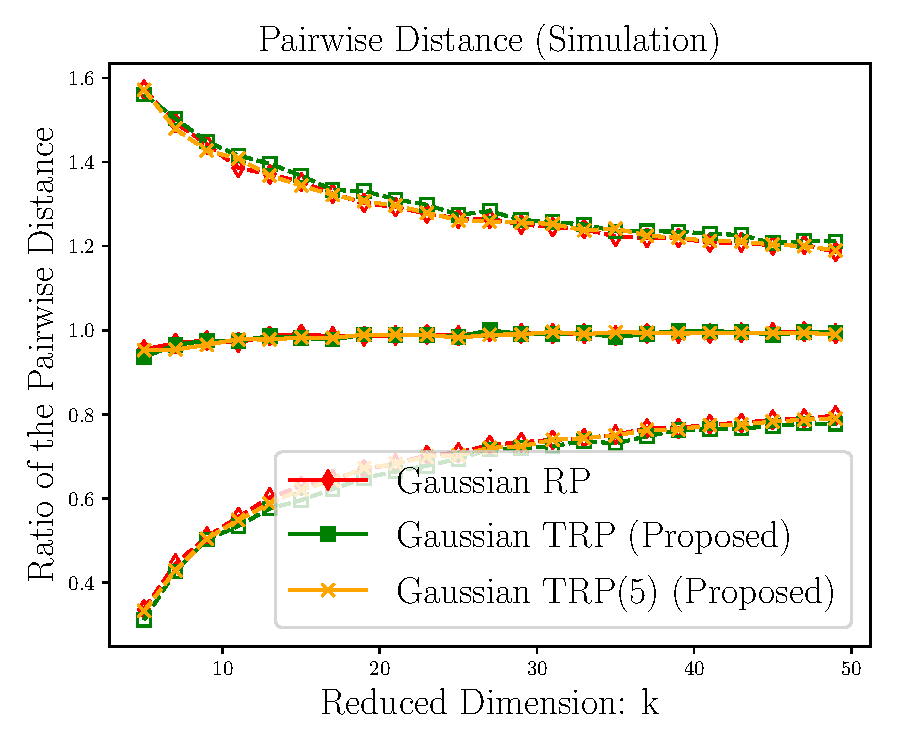
\includegraphics[scale = 0.3]{figure/dist_g_d2500.pdf}
	\end{subfigure}
	\begin{subfigure}{0.32\textwidth}
		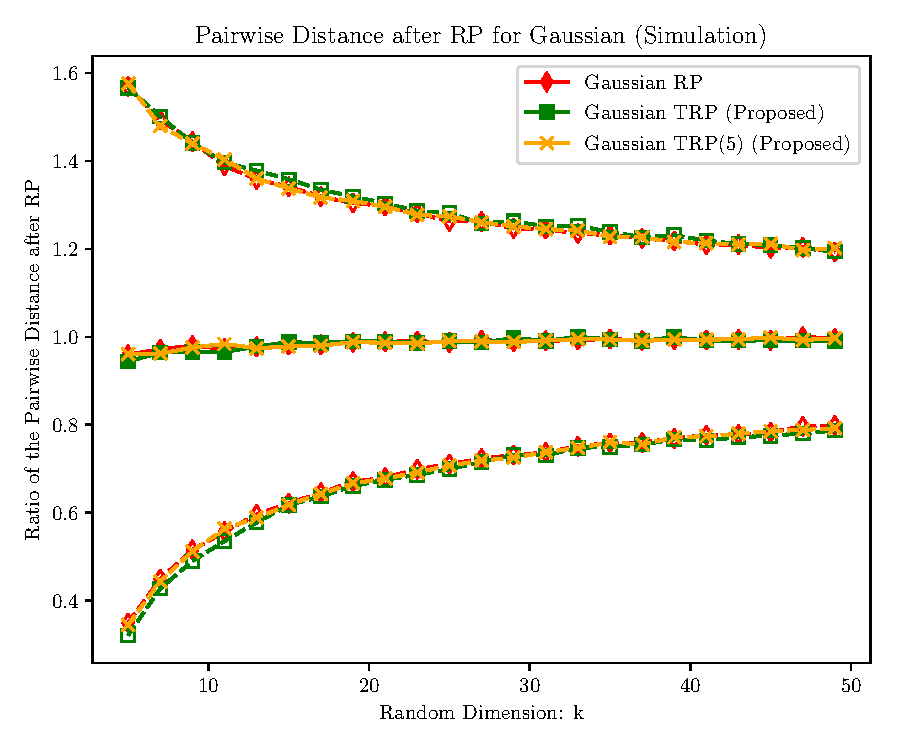
\includegraphics[scale = 0.3]{figure/dist_g_d10000.pdf}
	\end{subfigure}
	\begin{subfigure}{0.32\textwidth}
		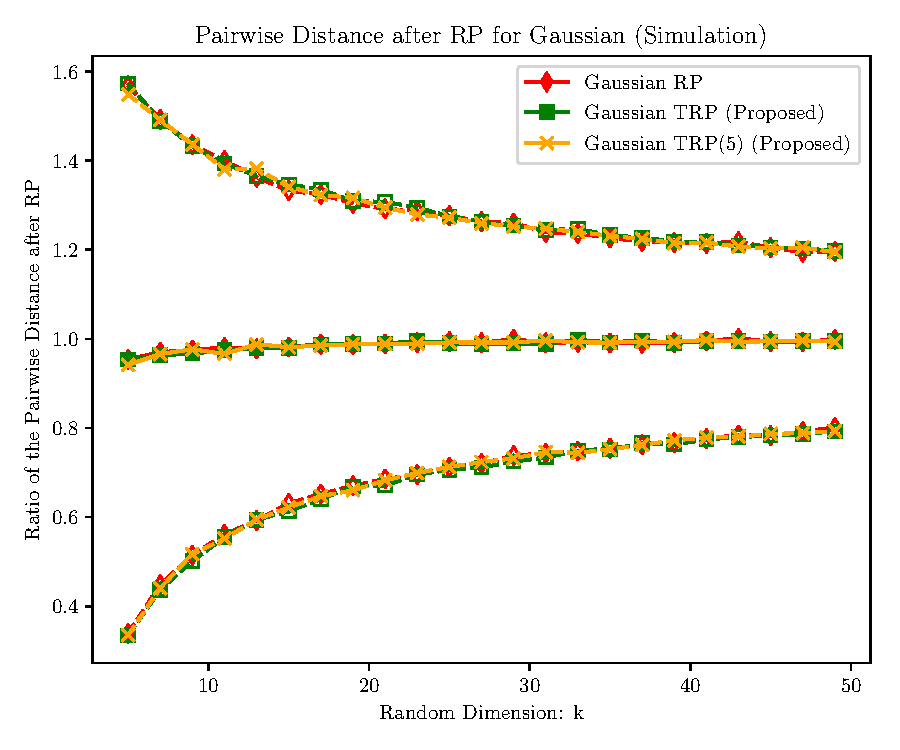
\includegraphics[scale = 0.3]{figure/dist_g_d40000.pdf}
	\end{subfigure}
	\\
	\caption{Average ratio of the pairwise distance for simulation data using Gaussian RP: \textit{The  plots correspond to the simulation for Gaussian RP, TRP, $\textup{TRP}_5$ respectively with $n = 20, d = 2500, 10000, 40000$ and each data vector comes from $N(\mathbf{0}, \mathbf{I})$. The dashed line represents the error bar 2 standard deviation away from the average ratio.}} 
	\label{fig:gaussian}
\end{figure}

\begin{figure*}[ht!]
	\centering
	\begin{subfigure}{0.32\textwidth}
		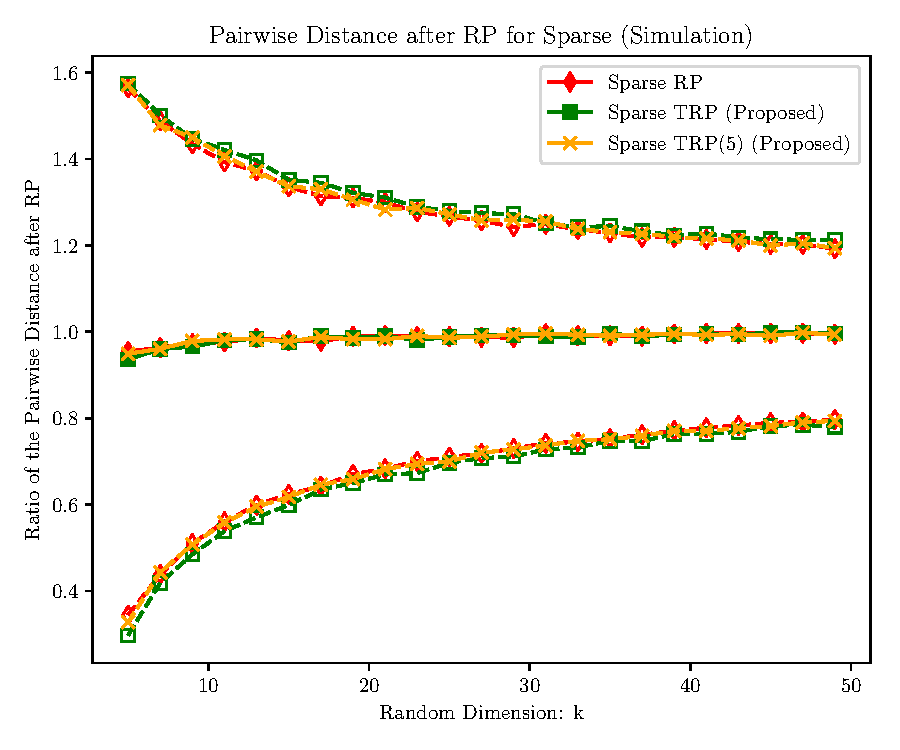
\includegraphics[scale = 0.3]{figure/dist_sp0_d2500.pdf}
	\end{subfigure}
	\begin{subfigure}{0.32\textwidth}
		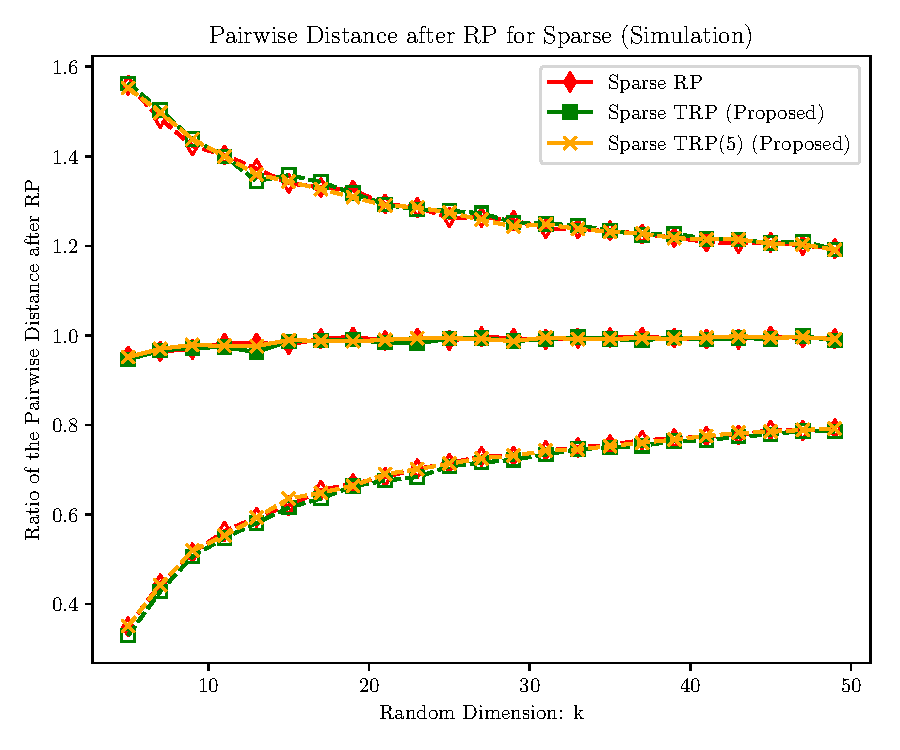
\includegraphics[scale = 0.3]{figure/dist_sp0_d10000.pdf}
	\end{subfigure}
	\begin{subfigure}{0.32\textwidth}
		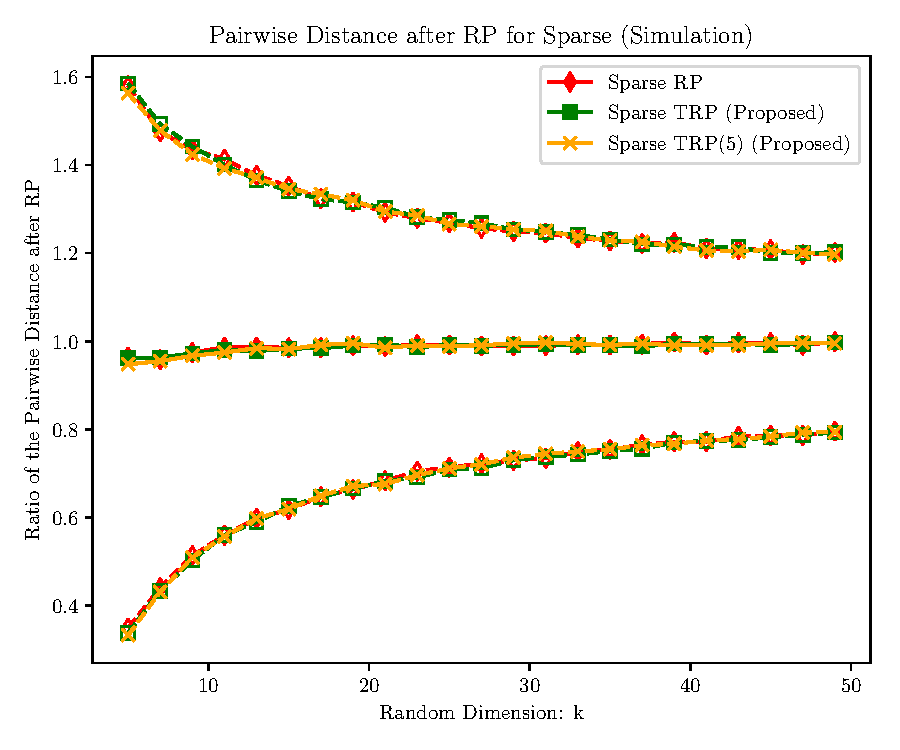
\includegraphics[scale = 0.3]{figure/dist_sp0_d40000.pdf}
	\end{subfigure}\\
	\caption{Average ratio of the pairwise distance for simulation data using Sparse RP: \textit{The  plots correspond to the simulation for Sparse RP, TRP, $\textup{TRP}_5$ respectively with $n = 20, d = 2500, 10000, 40000$ and each data vector comes from $N(\mathbf{0}, \mathbf{I})$. The dashed line represents the error bar 2 standard deviation away from the average ratio.}} 
	\label{fig:sparse}
\end{figure*}

\begin{figure*}[ht!] 
	\centering
	\begin{subfigure}{0.32\textwidth}
		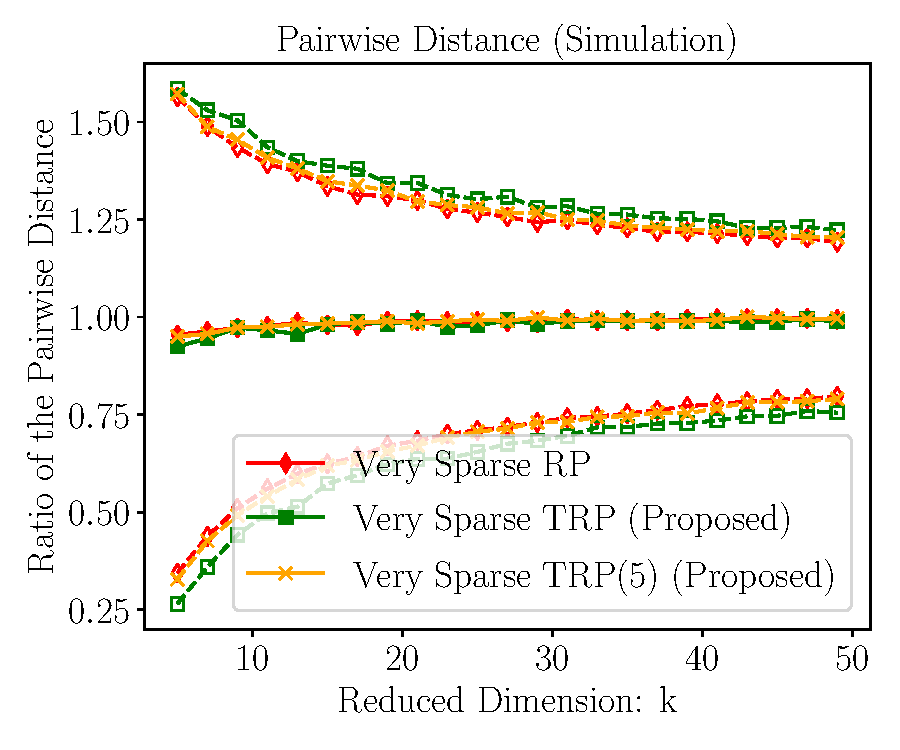
\includegraphics[scale = 0.3]{figure/dist_sp1_d2500.pdf}
	\end{subfigure}
	\begin{subfigure}{0.32\textwidth}
		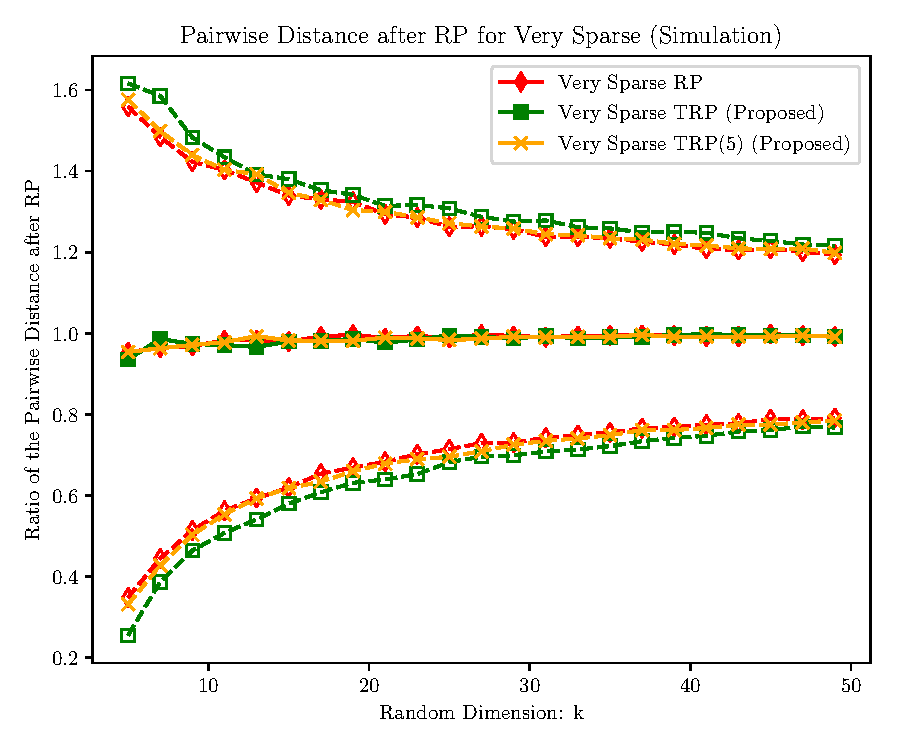
\includegraphics[scale = 0.3]{figure/dist_sp1_d10000.pdf}
	\end{subfigure}
	\begin{subfigure}{0.32\textwidth}
		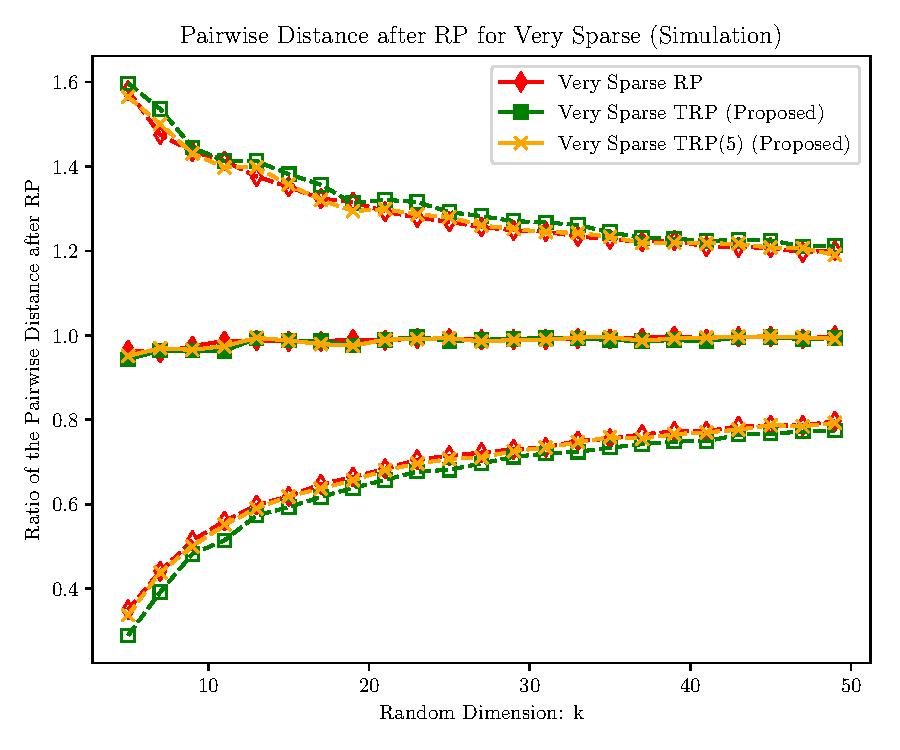
\includegraphics[scale = 0.3]{figure/dist_sp1_d40000.pdf}
	\end{subfigure}\\
	\caption{Average ratio of the pairwise distance for simulation data using Very Sparse RP: \textit{The plots correspond to the simulation for Very Sparse RP, TRP, $\textup{TRP}_5$ respectively with $n = 20, d = 2500, 10000, 40000$ and each data vector comes from $N(\mathbf{0}, \mathbf{I})$. The dashed line represents the error bar 2 standard deviation away from the average ratio.}} 
	\label{fig:very_sparse}
\end{figure*}

\begin{figure*}[ht!] 
	\centering
	\begin{subfigure}{0.32\textwidth}
		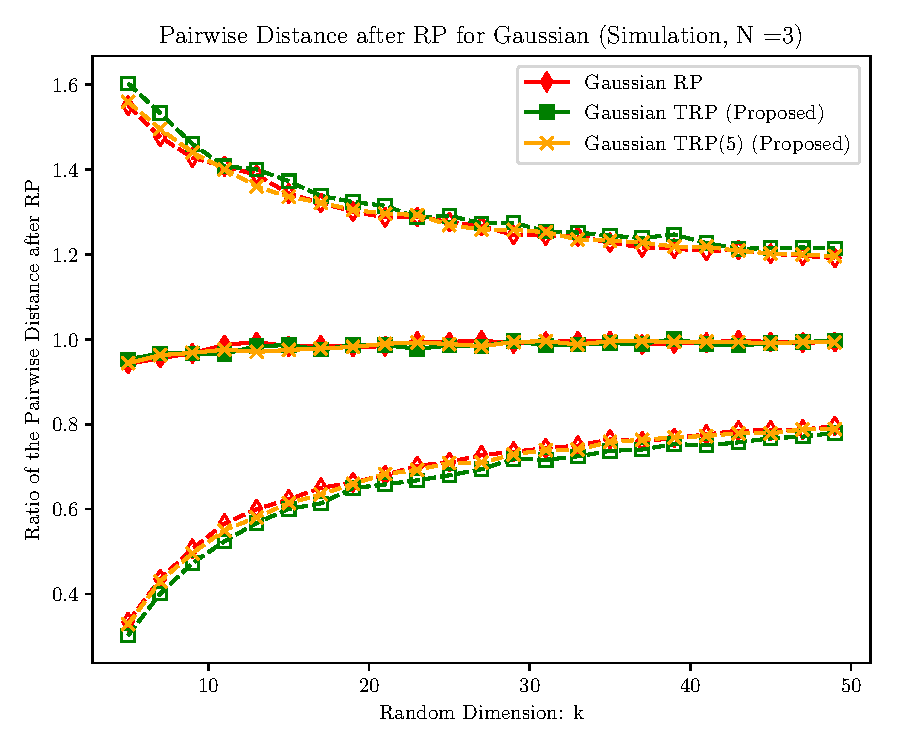
\includegraphics[scale = 0.3]{figure/dist_g_d125000.pdf}
	\end{subfigure}
	\begin{subfigure}{0.32\textwidth}
		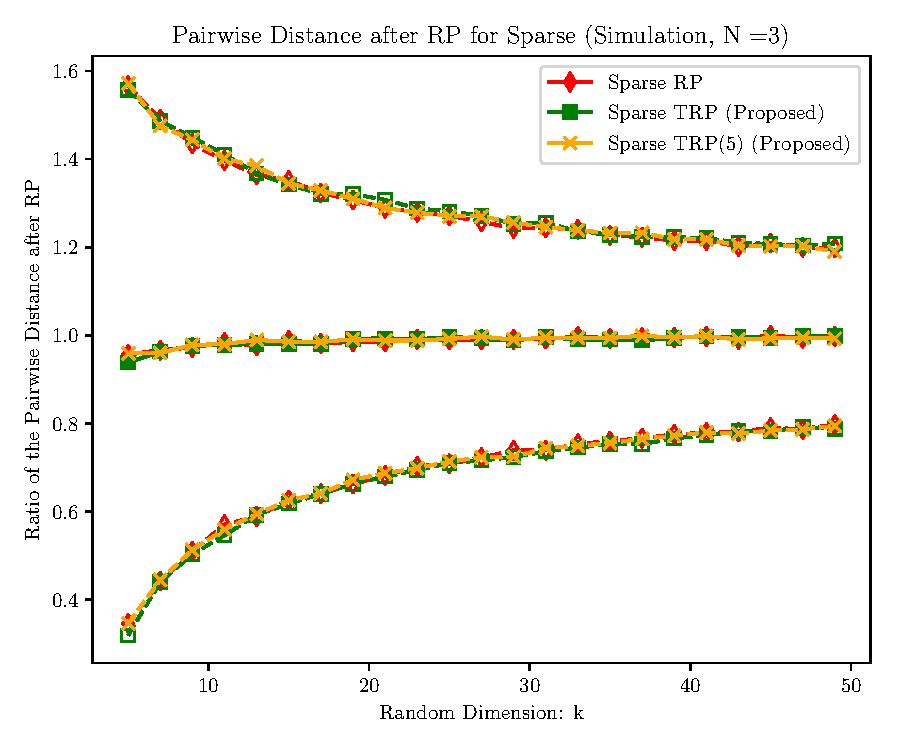
\includegraphics[scale = 0.3]{figure/dist_sp0_d125000.pdf}
	\end{subfigure}
	\begin{subfigure}{0.32\textwidth}
		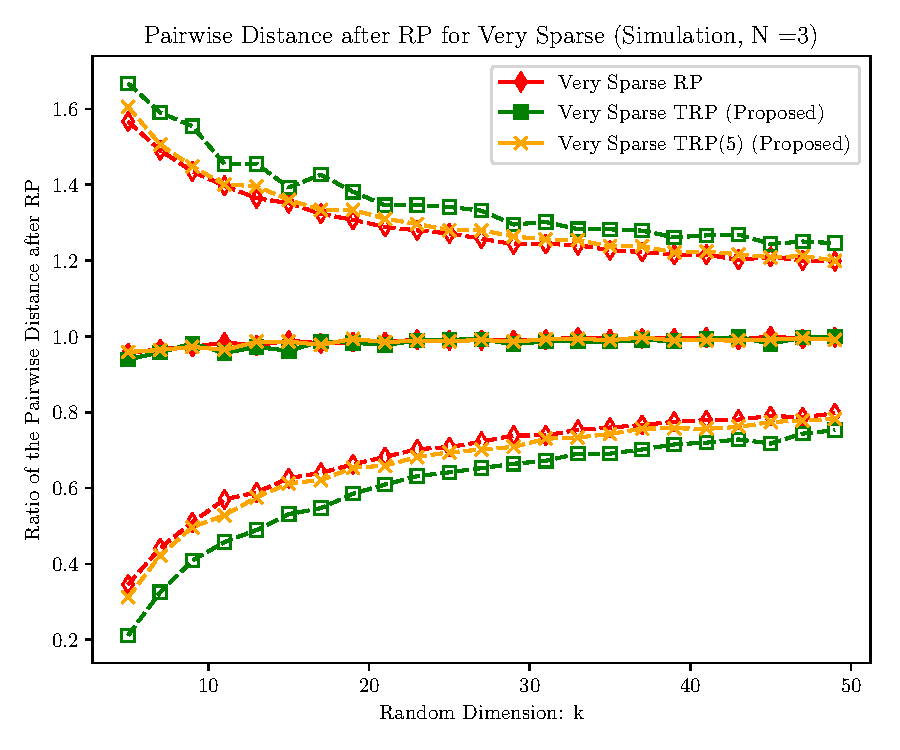
\includegraphics[scale = 0.3]{figure/dist_sp1_d125000.pdf}
	\end{subfigure}\\
	\caption{Average ratio of the pairwise distance for simulation data using: \textit{The plots correspond to the simulation for Gaussian, Sparase, Very Sparse RP, TRP, $\textup{TRP}_5$ respectively with $n = 20, d = d_1d_2d_3 = 50 \times 50 \times 50 = 125000$ and each data vector comes from $N(\mathbf{0}, \mathbf{I})$. The dashed line represents the error bar 2 standard deviation away from the average ratio.}} 
	\label{fig:triple_krao}
\end{figure*}


\paragraph{Pairwise Cosine Similarity Estimation} 
The second experiment is to estimate the pairwise cosine similarity, i.e. $\frac{\mathbf{x}_i \cdot \mathbf{x}_j}{\|\mathbf{x}_i\|_2 \|\mathbf{x}_j\|_2}$ for $\mathbf{ x}_i, \mathbf{x}_j$. We use both the simulation data ($d = 10000$) and the MNIST data ($d = 784, n = 60000$). We experiment with Gaussian, Sparse, Very Sparse RP, TRP, and $\textup{TRP}_5$ with the same setting as above ($k = 50$). We evaluate the performance by the average root mean square error (RMSE). The results is given in Table  \ref{tbl:mnist_inner_prod}, \ref{tbl:sim_inner_prod}.  

\begin{table}[ht!]
\centering
\begin{tabular}{l|l|l|l}
       & Gaussian        & Sparse          & Very Sparse     \\ \hline
RP     & 0.1409 (0.0015) & 0.1407 (0.0013) & 0.1412 (0.0014) \\ \hline
TRP    & 0.1431 (0.0016) & 0.1431 (0.0015) & 0.1520 (0.0033) \\ \hline
$\textup{TRP}_5$ & 0.1412 (0.0012) & 0.1411 (0.0015) & 0.1427 (0.0014)
\end{tabular}
\caption{RMSE for the estimate of the pairwise inner product of the simulation data ($d = 10000, k = 50, n = 100 $), where standard error is in the parentheses.
}\label{tbl:sim_inner_prod}
\end{table}

\section{Appendix: Finite Sample Bound}
\begin{definition}
	\label{def:generalized-sub-exponential-mc}
	A random variable $x$ is said to satisfy the generalized-sub-exponential moment condition with constant $\alpha$, if for general positive integer $k$, there exists a general constant $C$(not depending on k), s.t. 
	\begin{equation}
	\mathbb{E} |x|^k \le (Ck)^{k \alpha}
	\end{equation}
\end{definition}



\subsection*{Proof for Proposition \ref{prop: N-2-bound}}
\begin{proof}
	From now on, with losing generality, we will assume $\|x\|=1$.  Let 
	\begin{equation}
	\mathbf{y}= \frac{1}{\sqrt{k}}(\mathbf{A}_1 \odot \mathbf{A}_2)^\top \mathbf{x}, \nonumber
	\end{equation}
	Lemma \ref{lemma: norm-preserve} asserts that $\mathbb{E}\|\mathbf{y}\|^2_2= \|\mathbf{x}\|^2_2$ (conditions in lemma \ref{lemma: norm-preserve} naturally hold for iid random variables in our setting). The key observation is that $y_i, i\in [k]$ is quadratic form of elements of $\mathbf{A}_i, i=1,2$. Then as quadratic form of sub-Gaussian variables, $y_i$ are identically independently distributed generalized sub-exponential random variable. Then we could use Hanson-Wright inequality to determine the constants in moments condition \ref{def:generalized-sub-exponential-mc} which shall present tighter bound compared to directly citing results of linear combination of sub-exponential random variable defined in \eqref{def:generalized-sub-exponential-mc}
	
	
	We aim to write $y_i$ as a quadratic form of $\mathbf{z}_i:=[\mathop{\mathbf{vec}}(\mathbf{A}_{1}(\cdot,i)); \mathop{\mathbf{vec}}(\mathbf{A}_{2}(\cdot,i))]$. Also, for convenience, we partition $\mathbf{x}$ into $d_1$ sub-vectors with equal length $d_2$ i.e., $\mathbf{x} = [\mathbf{x}_1; \cdots; \mathbf{x}_{d_1}]$. To make it clear, we consider writing $y_1$ as quadratic form of $\mathbf{z}_1$ first.  
	\begin{equation}
	y_1 = \langle [\mathbf{A}_{1}(1,1) \mathbf{A}_{2}(\cdot,1); \cdots; \mathbf{A}_{1}(d_1,1) \mathbf{A}_{2}(\cdot,1)], [\mathbf{x}_1;\cdots; \mathbf{x}_{d_1}]\rangle
	\nonumber 
	\end{equation}
	which indicates that we could write
	\begin{equation}
	y_1 = \mathbf{z}^\top_1
	\mathbf{M}\mathbf{z}_1, \nonumber
	\end{equation}
	where 
	\begin{equation}
	\mathbf{M} = \begin{bmatrix}
	\mathbf{0} & \mathbf{D}\\
	\mathbf{0} & \mathbf{0}
	\end{bmatrix}  ~~
	\mathbf{D} = \begin{bmatrix}
	\mathbf{x}_1^\top \\
	\vdots \\
	\mathbf{x}_{d_1}^\top.  \nonumber
	\end{bmatrix}
	\end{equation}
	It is easy to see that $\|\mathbf{M}\| \le \|\mathbf{D}\| \le \|\mathbf{D}\|_F = \|\mathbf{M}\|_F = 1$ by assuming $\|\mathbf{x}\| = 1$. Then applying the Hanson Wright inequality in Lemma \ref{lemma:hanson_wright}, we could have for any positive number $\eta$, there exists a general constant $c_1$ s.t. 
	\begin{equation}
	\begin{aligned}
	\mathbb{P}(|y_i|\ge \eta) & \le 2\exp\left[-c_1\min\left\{ -\frac{\eta}{\varphi_2^2 \|M\|} ,  \frac{\eta^2}{\varphi_2^4 \|M\|^2_F} \right\} \right] \\
	& \le  2\exp\left[-c_1\min\left\{ -\frac{\eta}{\varphi_2^2} ,  \frac{\eta^2}{\varphi_2^4 } \right\} \right].  \nonumber
	\end{aligned}
	\end{equation}
	Then by Lemma \ref{lemma:hanson-wright-sub-exponential}, we could find a constant $C$ depending on sub-Gaussian norm and general constant $c_1$ s.t.
	\begin{equation}
	\mathbb{E} |y_i|^k \le (Ck)^k, \nonumber 
	\end{equation}
	where in fact we could give the explicit form of $C$ as 
	\begin{equation}\label{eq:constant_in-sub-exponential}
	C = 1+ \frac{c_1}{\min\left\{\varphi_2^2, \varphi_2^4\right\}}. 
	\end{equation}
	Notice $y_i$ has mean zero and variance 1 (assuming $\|x\|=1$),  then apply Lemma \ref{lemma:hanson-wright-sub-exponential-moment}, we could assert that there exists a general constant $c_2$
	\begin{equation}
	\begin{aligned}
	& \mathbb{P}\left(\left|\frac{1}{k} \mathbf{y}^\top \mathbf{I}_{k,k} \mathbf{y}-1 \right|\ge \epsilon\right )  \le C\exp\left( - c_2 \left[\sqrt{k}\epsilon\right]^{1/4} \right),
	\nonumber 
	\end{aligned}
	\end{equation}
	where $C$ is defined in \eqref{eq:constant_in-sub-exponential} and we use the fact $\alpha=1$ in our case which is defined in moments condition. 
	
	
	
	
\end{proof}


\begin{lem}
\label{lemma:inner-product}
For a linear mapping from $\mathbb{R}^d\rightarrow \mathbb{R}^k$: $f(\mathbf{x}) = \frac{1}{\sqrt{k}}\mathbf{\Omega x}$, 
\begin{equation}
\label{eq:inner-bound}
\mathbb{P}(|\langle f(\mathbf{x}), f(\mathbf{y})\rangle - \langle \mathbf{x}, \mathbf{y}\rangle|\ge \epsilon |\langle \mathbf{x}, \mathbf{y}\rangle|) \le 2\sup_{\mathbf{x}\in \mathbb{R}^{d}}\mathbb{P}(| \|f(\mathbf{x})\|^2-\|\mathbf{x}\|^2|\ge \epsilon \|\mathbf{x}\|_2^2).\nonumber
\end{equation}
\end{lem}

\begin{proof}
Since $f$ is a linear mapping, we have
\[
4f(\mathbf{x})f(\mathbf{y}) = \|f(\mathbf{x}+\mathbf{y})\|^2_2-  \|f(\mathbf{x}-\mathbf{y})\|^2_2.
\]
Consider the event

\begin{equation}
\begin{aligned}
 &\mathcal{A} _1=  \left\{ |\|f(\mathbf{x}+\mathbf{y})\|^2_2-\|\mathbf{x}+\mathbf{y}\|^2_2|\ge \epsilon \|\mathbf{x}+\mathbf{y}\|_2^2 \right\}\\
 &\mathcal{A} _2=  \left\{ | \|f(\mathbf{x}-\mathbf{y})\|^2_2-\|\mathbf{x}-\mathbf{y}\|^2_2|\ge \epsilon \|\mathbf{x}-\mathbf{y}\|_2^2 \right\} \nonumber
 \end{aligned}
 \end{equation}
 
 On the event $\mathcal{A}_1^\complement \cap\mathcal{A}_2^\complement$, 
 \[
 4f(\mathbf{x})f(\mathbf{y})  \ge (1-\epsilon) (\mathbf{x}+\mathbf{y})^2 - (1+\epsilon) (\mathbf{x}-\mathbf{y})^2 = 4 \langle \mathbf{x}, \mathbf{y}\rangle -2\epsilon (\|\mathbf{x}\|^2+\|\mathbf{y}\|^2),
 \]
 noticing $\|\mathbf{x}\|^2+\|\mathbf{y}\|^2\ge 2\langle \mathbf{x},  \mathbf{y}\rangle$, and by similar argument on the other side of the inequality, we could claim that 
\[
\left\{|\langle f(\mathbf{x}), f(\mathbf{y})\rangle - \langle \mathbf{x}, \mathbf{y}\rangle|\ge \epsilon |\langle \mathbf{x}, \mathbf{y}\rangle|\right\} \subseteq  \mathcal{A}_1 \cup \mathcal{A}_2. 
\]
Then we finish the proof by simply applying an union bound of two events. 
\end{proof}
\begin{remark}
The key element of classic random projections is the dimension-free bound. Similarly, according to Prop. \ref{prop: N-2-bound}, our TRP has a norm preservation bound independent of the particular vector  $\mathbf{x}$ and dimension $d$ and thus a dimension-free inner product preservation bound according to Lemma \ref{eq:inner-bound}. 
\end{remark}



\section{Technical Lemmas}
In this section, we list some technical lemmas we use in this paper. All of them are about tail probability of sub-Gaussian or generalized sub-exponential variables. 

\begin{definition}
	\label{def:sub-gaussian}
	A random variable $x$ is called sub-Gaussian if $\mathbb{E} |x|^p = \mathcal{O}(p^{p/2})$ when $p\rightarrow \infty$. With this, we define sub-Gaussian norm for $x$ (less than infinity) as 
	\begin{equation}
	\|x\|_{\varphi_2} = \sup_{p\ge 1} p^{-1/2} (\mathbb{E} |x|^p)^{1/p}. 
	\end{equation}
\end{definition}

Note that for Bernoulli random variable, i.e., $\{-1,1\}$ with prob. $\{\frac{1}{2},\frac{1}{2} \}$,  $\varphi_2=1$; any bounded random variable with absolute value less than $M>0$ has $\varphi_2\le M$.  For standard Gaussian random variable, $\varphi_2=1$. 



\begin{lem}
\label{lemma:hanson_wright}
(Hanson-Wright Inequality) Let $\mathbf{x} = (x_1,\cdots , x_n)\in \mathbb{R}^n$ be a random
vector with independent components $X_i$ which satisfies $\mathbb{E} \mathbf{x}_i = 0$ and $\varphi_2(x_1)\le K$. Let $A$
be an $n\times n$ matrix. Then, for every $\eta \ge 0$, there exists a general constant $c$ s.t.
\begin{equation}
\mathbb{P}\left(|\mathbf{x^\top A x} - \mathbb{E}\mathbf{x^\top A x}|\ge \eta\right)\le 2\exp\left[-c\min\left\{\frac{\eta}{K^2\|A\|}, \frac{\eta^2}{\|A\|_F^2 K^4}\right\}\right]. \nonumber
\end{equation}
\end{lem}

\begin{proof}
	Please refer to \cite{rudelson2013hanson}
\end{proof}



\begin{lem}
\label{lemma:hanson-wright-sub-exponential}
Let $\mathbf{x}$ be a random
variable whose tail probability satisfies for every $\eta \ge 0$, there exists a constant $c_1$ s.t. 
\begin{equation}
\mathbb{P}\left(|x|\ge \eta\right)\le 2\exp\left[-c_1\min\left(\eta,  \eta^2\right)\right]. \nonumber
\end{equation}
Then for any $k\ge 1$, $x$ satisfies generalized sub-exponential moment condition \ref{def:generalized-sub-exponential-mc} with $\alpha = 1$, i.e., 
\begin{equation}
\mathbb{E} |x|^k \le (Ck)^k, \nonumber
\end{equation}\label{eq:sub-exponential-moment-condition}
where $C= 1+\frac{1}{c_1}$.
\end{lem}
\begin{proof} 
\begin{equation}
\begin{aligned}
&\mathbb{E} |x|^k =  \int_{0}^1 kx^{k-1} 2\exp[-c_1x^2]dx + \int_{1}^\infty kx^{k-1} 2\exp[-c_1x]dx \\ 
&\le 1+ + \frac{1}{c_1^k}\int_{0}^\infty ky^{k-1} 2\exp[-y]dy\\
&= 1+ \frac{1}{c_1^k} k\Gamma(k-1)\le \left[1+\frac{1}{c_1^k}\right] k^k.
\end{aligned}
\end{equation}
Noticing $\left[1+\frac{1}{c_1^k}\right]^{1/k} \le 1+\frac{1}{c_1}$, we finish the proof. 
\end{proof}


\begin{lem}\label{lemma:hanson-wright-sub-exponential-moment}
	For a random vector $\mathbf{x}$ with each element independent and identically distributed with mean zero and variance 1, suppose each element of $\mathbf{x}$
	satisfies generalized sub-exponential moment condition as in \eqref{eq:sub-exponential-moment-condition}, that there exists a general constant $C$ s.t.  $\mathbb{E} |x_1|^k \le (Ck)^{\alpha k}$. Then for any matrix $\mathbf{A} \in \mathbb{R}^{n \times n}$, there exists a general constant $c_1$
	\begin{equation}
		\mathbb{P}\left(\left|\mathbf{x}^\top \mathbf{A} \mathbf{x} - \mathbb{E} \mathbf{x}^\top \mathbf{A} \mathbf{x} \right| \ge \eta \right)\le  C \exp\left(-c_1\left[\frac{\eta}{\|A\|_F}\right]^{1/(2(1+\alpha))}\right) . \nonumber
	\end{equation}
\end{lem}
\begin{proof}
	The proof is directly from Lemma 8.3 in \cite{buhler2002finding} and we change the statement on generalized sub-exponential R.V. directly to the statement on the moment condition. 
\end{proof}





%\clearpage
\end{appendices}


\end{document}
